\documentclass[
	12pt,
	oneside,
	a4paper,
	brazilian
]{abntex2}

\usepackage{cmap}
\usepackage{lmodern}
\usepackage[utf8]{inputenc}
\usepackage[T1]{fontenc}
\usepackage{booktabs}
\usepackage{tabularx}
\usepackage{float}
\usepackage{graphicx}
\usepackage{xcolor}
\usepackage{microtype}
\usepackage{indentfirst}
\usepackage{enumitem}

\definecolor{azulunirv}{RGB}{15,44,89}
\definecolor{verdeagro}{RGB}{21,128,61}
\definecolor{cinzafundo}{RGB}{245,247,250}

\hypersetup{
	pdftitle={AgroContas — Documento de Especificação de Requisitos}, 
	pdfauthor={Equipe de Desenvolvimento AgroContas},
	pdfsubject={Engenharia de Requisitos - Disciplina DOO},
	pdfcreator={LaTeX with abnTeX2},
	colorlinks=true,
	linkcolor=azulunirv,
	citecolor=azulunirv,
	filecolor=magenta,
	urlcolor=azulunirv,
	bookmarksdepth=4
}

\setlength{\parindent}{1.3cm}
\setlength{\parskip}{0.2cm}

\titulo{AGROCONTAS — SISTEMA DE GESTÃO FINANCEIRA RURAL\\Documento de Especificação de Requisitos}
\autor{Equipe de Desenvolvimento AgroContas}
\local{Rio Verde — GO}
\data{2026}
\instituicao{Universidade de Rio Verde — UniRV\\Faculdade de Engenharia de Software / Ciência da Computação\\Disciplina de Desenvolvimento Orientado a Objetos (DOO)}
\tipotrabalho{Relatório Técnico de Requisitos de Software}
\preambulo{Documento de Especificação de Requisitos apresentado como requisito parcial de avaliação na disciplina de Desenvolvimento Orientado a Objetos (DOO) da Universidade de Rio Verde (UniRV).}

\begin{document}
\selectlanguage{brazilian}
\frenchspacing

% ==========================================================
% CAPA E FOLHA DE ROSTO
% ==========================================================
\imprimircapa
\imprimirfolhaderosto

% ==========================================================
% HISTÓRICO DE ALTERAÇÕES
% ==========================================================
\clearpage
\begin{center}
	{\Large\bfseries HISTÓRICO DE ALTERAÇÕES}
\end{center}
\vspace{1cm}

\noindent Em estrito cumprimento às diretrizes acadêmicas da disciplina, a presente documentação é formalmente mantida na \textbf{Versão 1.0}, registrando o ciclo oficial de homologação das especificações e requisitos funcionais.

\vspace{0.5cm}

\begin{table}[H]
	\centering
	\small
	\begin{tabularx}{\textwidth}{p{2.5cm} p{2cm} p{6.5cm} X}
		\toprule
		\textbf{Data} & \textbf{Versão} & \textbf{Descrição} & \textbf{Autor} \\
		\midrule
		02/09/2026 & 1.0 & Elaboração oficial e consolidação da Especificação de Requisitos em conformidade com as diretrizes da disciplina de DOO/UniRV. Estruturação dos 7 Requisitos Funcionais, modelagem relacional de 5 entidades com integridade referencial, e inclusão de especificações completas com telas de listagem para operações de manutenção. & Equipe AgroContas \\
		\bottomrule
	\end{tabularx}
\end{table}

% ==========================================================
% SUMÁRIO
% ==========================================================
\clearpage
\tableofcontents*

% ==========================================================
% CORPO DO DOCUMENTO
% ==========================================================
\clearpage
\textual

\chapter{MISSÃO DO PRODUTO}

Para produtores rurais familiares e gestores do agronegócio que necessitam gerenciar receitas e despesas de sua propriedade de forma centralizada e sem atrito operacional, o \textbf{AgroContas} é uma solução de gestão financeira que auxilia no controle rigoroso de contas a pagar e contas a receber. 

Diferentemente de controles manuais em cadernos e planilhas desconexas — que exigem rotinas burocráticas e propensas a falhas de digitação —, o produto oferece praticidade e automação na captura de dados a partir de documentos em PDF (como faturas e Notas Fiscais Eletrônicas), gerenciando de forma transparente os fornecedores, as despesas/receitas classificadas, os títulos de contas, seus parcelamentos vinculados e a respectiva quitação financeira através de uma interface visual amigável e acessível.

\chapter{LISTA DE FUNÇÕES}

A Tabela \ref{tab:funcoes} estabelece a lista oficial dos Requisitos Funcionais (RF) que compõem o escopo do produto \textbf{AgroContas}, devidamente padronizados no modelo de engenharia de software da disciplina.

\begin{table}[H]
	\centering
	\small
	\caption{Lista de Requisitos Funcionais do Sistema AgroContas}
	\label{tab:funcoes}
	\begin{tabularx}{\textwidth}{c p{5cm} X}
		\toprule
		\textbf{ID} & \textbf{Nome da Funcionalidade} & \textbf{Descrição do Requisito} \\
		\midrule
		\textbf{RF01} & Manter Fornecedor / Cliente & Permite cadastrar, consultar, alterar e desativar pessoas físicas e jurídicas que atuam como fornecedores de insumos/serviços ou clientes/titulares adquirentes da produção agrícola. \\
		\midrule
		\textbf{RF02} & Manter Despesas / Receitas & Gerencia as contas contábeis e categorias operacionais (ex.: adubos, defensivos, combustíveis, venda de grãos), padronizando a classificação dos lançamentos financeiros. \\
		\midrule
		\textbf{RF03} & Manter MovimentoContas & Registra os títulos principais de Contas a Pagar e Contas a Receber, associando o documento fiscal ao fornecedor, ao faturado e à categoria de despesa/receita. \\
		\midrule
		\textbf{RF04} & Manter MovimentoParcelas & Controla as parcelas vinculadas a cada conta cadastrada, gerenciando prazos de vencimento, valores fracionados e controle do saldo residual. \\
		\midrule
		\textbf{RF05} & Manter MovimentoFinanceiro (Quitação) & Registra as operações de quitação e liquidação financeira das parcelas (baixas totais ou parciais), informando data de pagamento, juros, descontos e comprovante. \\
		\midrule
		\textbf{RF06} & Fazer Upload do Documento & Provê interface para carregamento e envio de arquivos em formato PDF contendo faturas, boletos ou Notas Fiscais Eletrônicas (NF-e). \\
		\midrule
		\textbf{RF07} & Extrair Dados do Documento & Executa a análise e processamento do documento carregado, extraindo automaticamente dados cadastrais, datas, valores totais e parcelamentos para conferência. \\
		\bottomrule
	\end{tabularx}
\end{table}

\chapter{REQUISITOS DE QUALIDADE}

Os Requisitos Não-Funcionais e critérios de qualidade do sistema abrangem:

\begin{itemize}[leftmargin=1.5cm]
	\item \textbf{Usabilidade e Clareza}: A interface deve apresentar baixa carga cognitiva, orientando o usuário em tarefas sequenciais e objetivas.
	\item \textbf{Codificação Cromática}: Emprego de padrões visuais claros (Verde para Receitas/Valores Positivos e Vermelho/Laranja para Despesas e Contas Pendentes).
	\item \textbf{Feedback Imediato}: Apresentação de mensagens claras de validação em caso de campos obrigatórios não preenchidos ou falhas de comunicação.
	\item \textbf{Integridade Referencial}: Garantia de que nenhuma movimentação de conta, parcela ou quitação exista sem os vínculos consistentes com as entidades de origem.
	\item \textbf{Tempo de Resposta}: O processamento e extração de documentos em PDF deve retornar resposta estruturada para conferência em menos de 5 segundos em ambiente padrão de rede.
\end{itemize}

\chapter{METAS GERENCIAIS}

\begin{itemize}[leftmargin=1.5cm]
	\item \textbf{Investimento Máximo Estimado}: R\$ 35.000,00.
	\item \textbf{Prazo Máximo de Conclusão}: 4 meses (distribuídos em 8 sprints de desenvolvimento).
\end{itemize}

\chapter{OUTROS ASPECTOS}

\begin{itemize}[leftmargin=1.5cm]
	\item \textbf{Limitação de Escopo Legal}: O sistema tem finalidade gerencial e operacional de controle de fluxo de caixa rural. Não substitui sistemas fiscais com emissão de certificados digitais A1/A3 ou envio direto do SPED Fiscal à Receita Federal do Brasil.
\end{itemize}

\chapter{ESTIMATIVA DE PRAZO PARA A ELABORAÇÃO}

O cronograma detalhado de execução física do projeto foi modelado no software \textbf{GanttProject} e está detalhado na Tabela do \textbf{Anexo 1}, estimando-se 1 recurso técnico para especificação inicial e equipe de desenvolvimento para execução dos 7 módulos.

\chapter{ESPECIFICAÇÃO TÉCNICA DO PRODUTO}

\section{Arquitetura Estrutural do Sistema}

A Figura \ref{fig:arquitetura} apresenta a arquitetura em camadas do AgroContas, destacando o desacoplamento entre a camada de apresentação visual, controladores de rotas, camada de serviços de extração inteligente e camada de persistência relacional.

\begin{figure}[H]
	\centering
	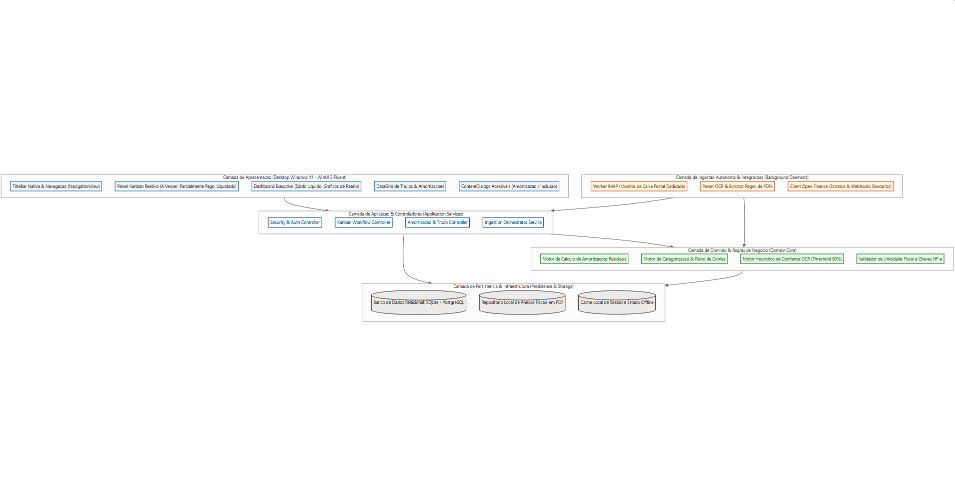
\includegraphics[width=0.88\textwidth]{assets/arquitetura.png}
	\caption{Diagrama de Arquitetura em Camadas do Sistema AgroContas}
	\label{fig:arquitetura}
\end{figure}

\section{Diagrama de Casos de Uso}

Em conformidade rigorosa com a orientação da disciplina, a Figura \ref{fig:casosdeuso} apresenta o Diagrama de Casos de Uso estruturado com os atores posicionados estritamente nas bordas externas e os \textbf{7 Casos de Uso no centro}, dentro do retângulo de limite do sistema (*System Boundary*).

\begin{figure}[H]
	\centering
	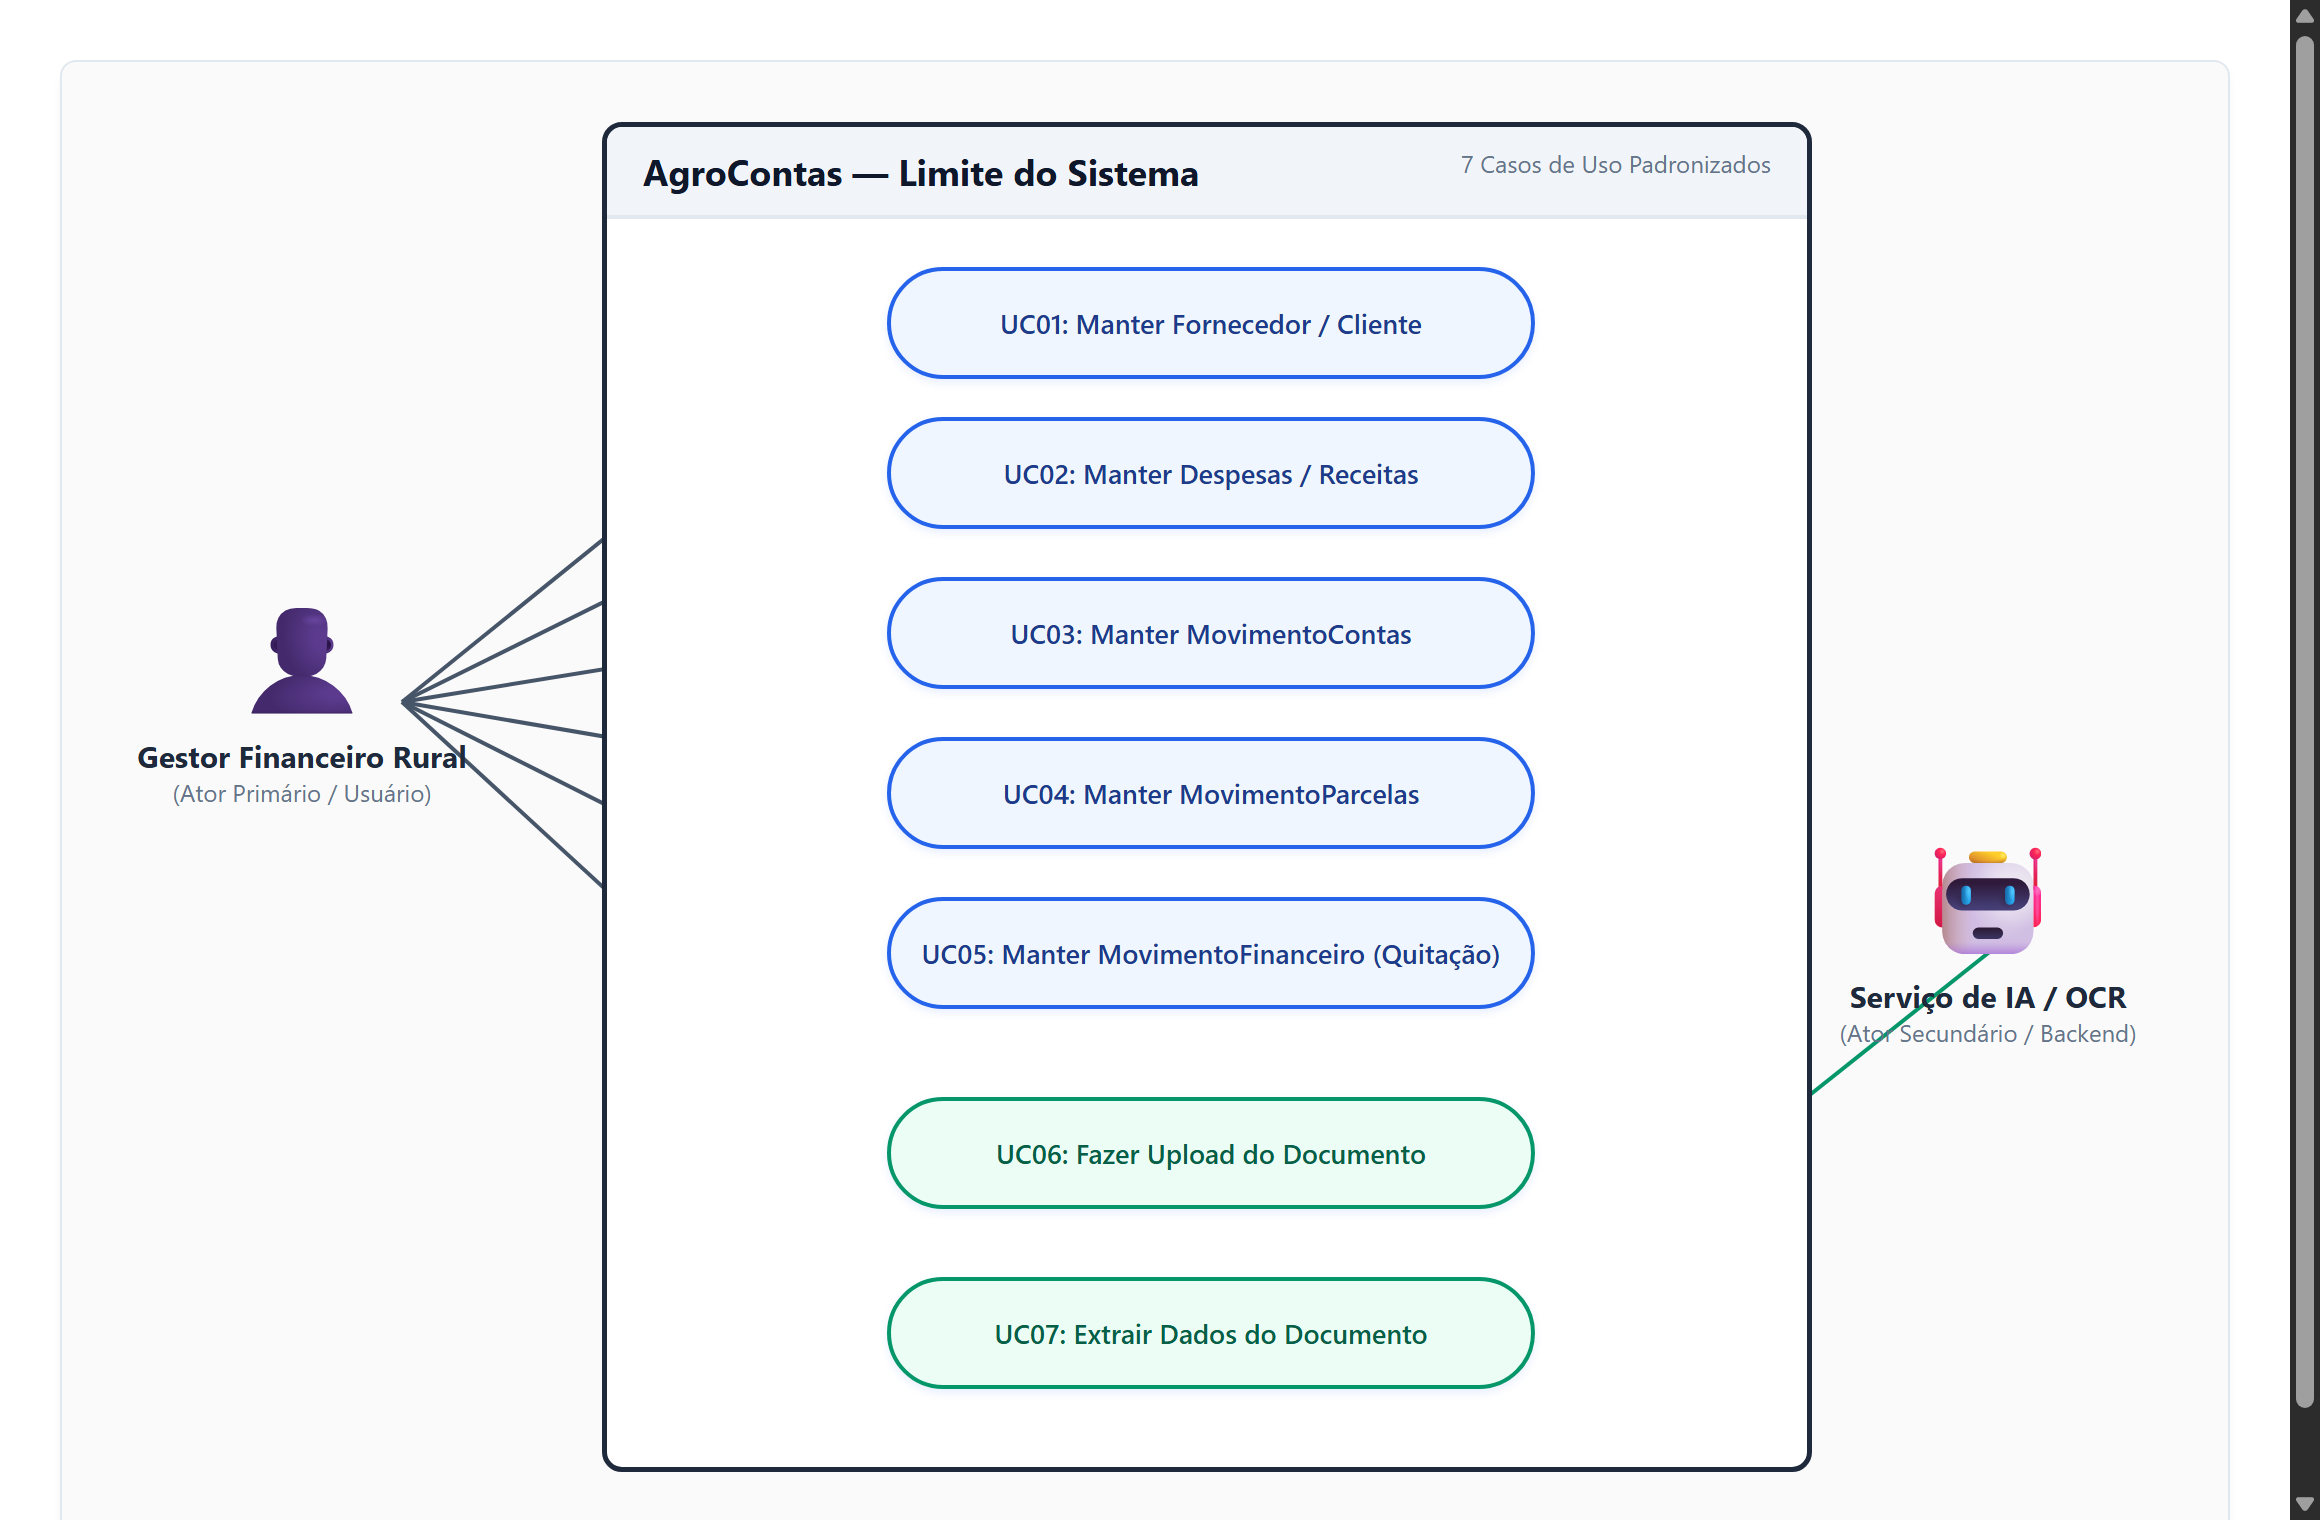
\includegraphics[width=0.95\textwidth]{assets/diagrama_caso_uso.png}
	\caption{Diagrama de Casos de Uso Padronizado (Bordas com Atores e Centro com os 7 RFs)}
	\label{fig:casosdeuso}
\end{figure}

\section{Detalhamento dos Casos de Uso}

Abaixo é apresentado o detalhamento formal de \textbf{todos os 7 requisitos funcionais} listados no Item 2, com a identificação de prioridade, dependências e materiais de apoio.

% --- UC01 ---
\vspace{0.3cm}
\noindent\fbox{\parbox{\textwidth}{
	\textbf{Requisito nº:} RF01 / UC01 — Manter Fornecedor / Cliente \\
	\textbf{Descrição:} Realiza o cadastro, consulta, alteração e inativação de parceiros comerciais (fornecedores de insumos agrícolas e clientes compradores da safra). \\
	\textbf{Prioridade:} Essencial \\
	\textbf{Dependências:} Nenhuma (entidade base primária). \\
	\textbf{Conflitos:} Nenhum. \\
	\textbf{Material de Apoio:} Diagrama de Casos de Uso, DER (Tabela FORNECEDOR\_CLIENTE), Protótipo de Tela (Anexo 2).
}}

% --- UC02 ---
\vspace{0.3cm}
\noindent\fbox{\parbox{\textwidth}{
	\textbf{Requisito nº:} RF02 / UC02 — Manter Despesas / Receitas \\
	\textbf{Descrição:} Mantém o catálogo de categorias contábeis e centros de custo operacionais da fazenda para classificação padronizada das entradas e saídas. \\
	\textbf{Prioridade:} Essencial \\
	\textbf{Dependências:} Nenhuma (entidade base primária). \\
	\textbf{Conflitos:} Nenhum. \\
	\textbf{Material de Apoio:} Diagrama de Casos de Uso, DER (Tabela DESPESAS\_RECEITAS), Protótipo de Tela (Anexo 2).
}}

% --- UC03 ---
\vspace{0.3cm}
\noindent\fbox{\parbox{\textwidth}{
	\textbf{Requisito nº:} RF03 / UC03 — Manter MovimentoContas \\
	\textbf{Descrição:} Gerencia a emissão e manutenção de títulos de Contas a Pagar e Contas a Receber, associando chaves estrangeiras com Despesas/Receitas, Fornecedor e Faturado. \\
	\textbf{Prioridade:} Essencial \\
	\textbf{Dependências:} RF01 (Fornecedor/Cliente), RF02 (Despesas/Receitas). \\
	\textbf{Conflitos:} Nenhum. \\
	\textbf{Material de Apoio:} Diagrama de Casos de Uso, DER (Tabela MOVIMENTO\_CONTAS), Protótipo de Tela (Anexo 2).
}}

% --- UC04 ---
\vspace{0.3cm}
\noindent\fbox{\parbox{\textwidth}{
	\textbf{Requisito nº:} RF04 / UC04 — Manter MovimentoParcelas \\
	\textbf{Descrição:} Registra e monitora o desdobramento dos títulos de contas em parcelas a prazo, calculando valores unitários, datas de vencimento e saldo pendente. \\
	\textbf{Prioridade:} Essencial \\
	\textbf{Dependências:} RF03 (MovimentoContas). \\
	\textbf{Conflitos:} Nenhum. \\
	\textbf{Material de Apoio:} Diagrama de Casos de Uso, DER (Tabela MOVIMENTO\_PARCELAS), Protótipo de Tela (Anexo 2).
}}

% --- UC05 ---
\vspace{0.3cm}
\noindent\fbox{\parbox{\textwidth}{
	\textbf{Requisito nº:} RF05 / UC05 — Manter MovimentoFinanceiro (Quitação) \\
	\textbf{Descrição:} Registra os pagamentos e baixas financeiras vinculados às parcelas, controlando liquidação contábil, encargos e formas de pagamento. \\
	\textbf{Prioridade:} Essencial \\
	\textbf{Dependências:} RF04 (MovimentoParcelas). \\
	\textbf{Conflitos:} Nenhum. \\
	\textbf{Material de Apoio:} Diagrama de Casos de Uso, DER (Tabela MOVIMENTO\_FINANCEIRO), Protótipo de Tela (Anexo 2).
}}

% --- UC06 ---
\vspace{0.3cm}
\noindent\fbox{\parbox{\textwidth}{
	\textbf{Requisito nº:} RF06 / UC06 — Fazer Upload do Documento \\
	\textbf{Descrição:} Disponibiliza interface para o usuário anexar arquivos digitais (PDF de notas fiscais, recibos e faturas) para iniciar a ingestão documental. \\
	\textbf{Prioridade:} Importante \\
	\textbf{Dependências:} Nenhuma. \\
	\textbf{Conflitos:} Nenhum. \\
	\textbf{Material de Apoio:} Diagrama de Casos de Uso, Diagrama de Sequência de Ingestão, Protótipo de Tela (Anexo 2).
}}

% --- UC07 ---
\vspace{0.3cm}
\noindent\fbox{\parbox{\textwidth}{
	\textbf{Requisito nº:} RF07 / UC07 — Extrair Dados do Documento \\
	\textbf{Descrição:} Processa o arquivo PDF submetido, reconhecendo entidades de fornecedor, cliente, valores, datas e despesas para pré-preenchimento das contas. \\
	\textbf{Prioridade:} Importante \\
	\textbf{Dependências:} RF06 (Fazer Upload do Documento). \\
	\textbf{Conflitos:} Nenhum. \\
	\textbf{Material de Apoio:} Diagrama de Casos de Uso, Diagrama de Sequência, Protótipo Split-View (Anexo 2).
}}

\section{Diagrama Entidade-Relacionamento (DER)}

A Figura \ref{fig:der} formaliza o Diagrama Entidade-Relacionamento rigorosamente ajustado para atender à modelagem relacional solicitada na avaliação do professor, compreendendo as 5 entidades e suas devidas chaves estrangeiras:

\begin{itemize}[leftmargin=1.5cm]
	\item \textbf{FORNECEDOR\_CLIENTE}: Cadastro central de titulares, fornecedores e clientes;
	\item \textbf{DESPESAS\_RECEITAS}: Plano de contas e classificação de despesas e receitas;
	\item \textbf{MOVIMENTO\_CONTAS}: Registro mestre de contas a pagar/receber, possuindo:
	\begin{itemize}
		\item Chave estrangeira com \textit{DESPESAS\_RECEITAS};
		\item Chave estrangeira com \textit{FORNECEDOR\_CLIENTE} (papel de Fornecedor/Credor);
		\item Chave estrangeira com \textit{FORNECEDOR\_CLIENTE} (papel de Faturado/Devedor/Titular);
	\end{itemize}
	\item \textbf{MOVIMENTO\_PARCELAS}: Parcelamento associado via chave estrangeira com \textit{MOVIMENTO\_CONTAS};
	\item \textbf{MOVIMENTO\_FINANCEIRO}: Registro de quitação e pagamentos associado via chave estrangeira com \textit{MOVIMENTO\_PARCELAS}.
\end{itemize}

\begin{figure}[H]
	\centering
	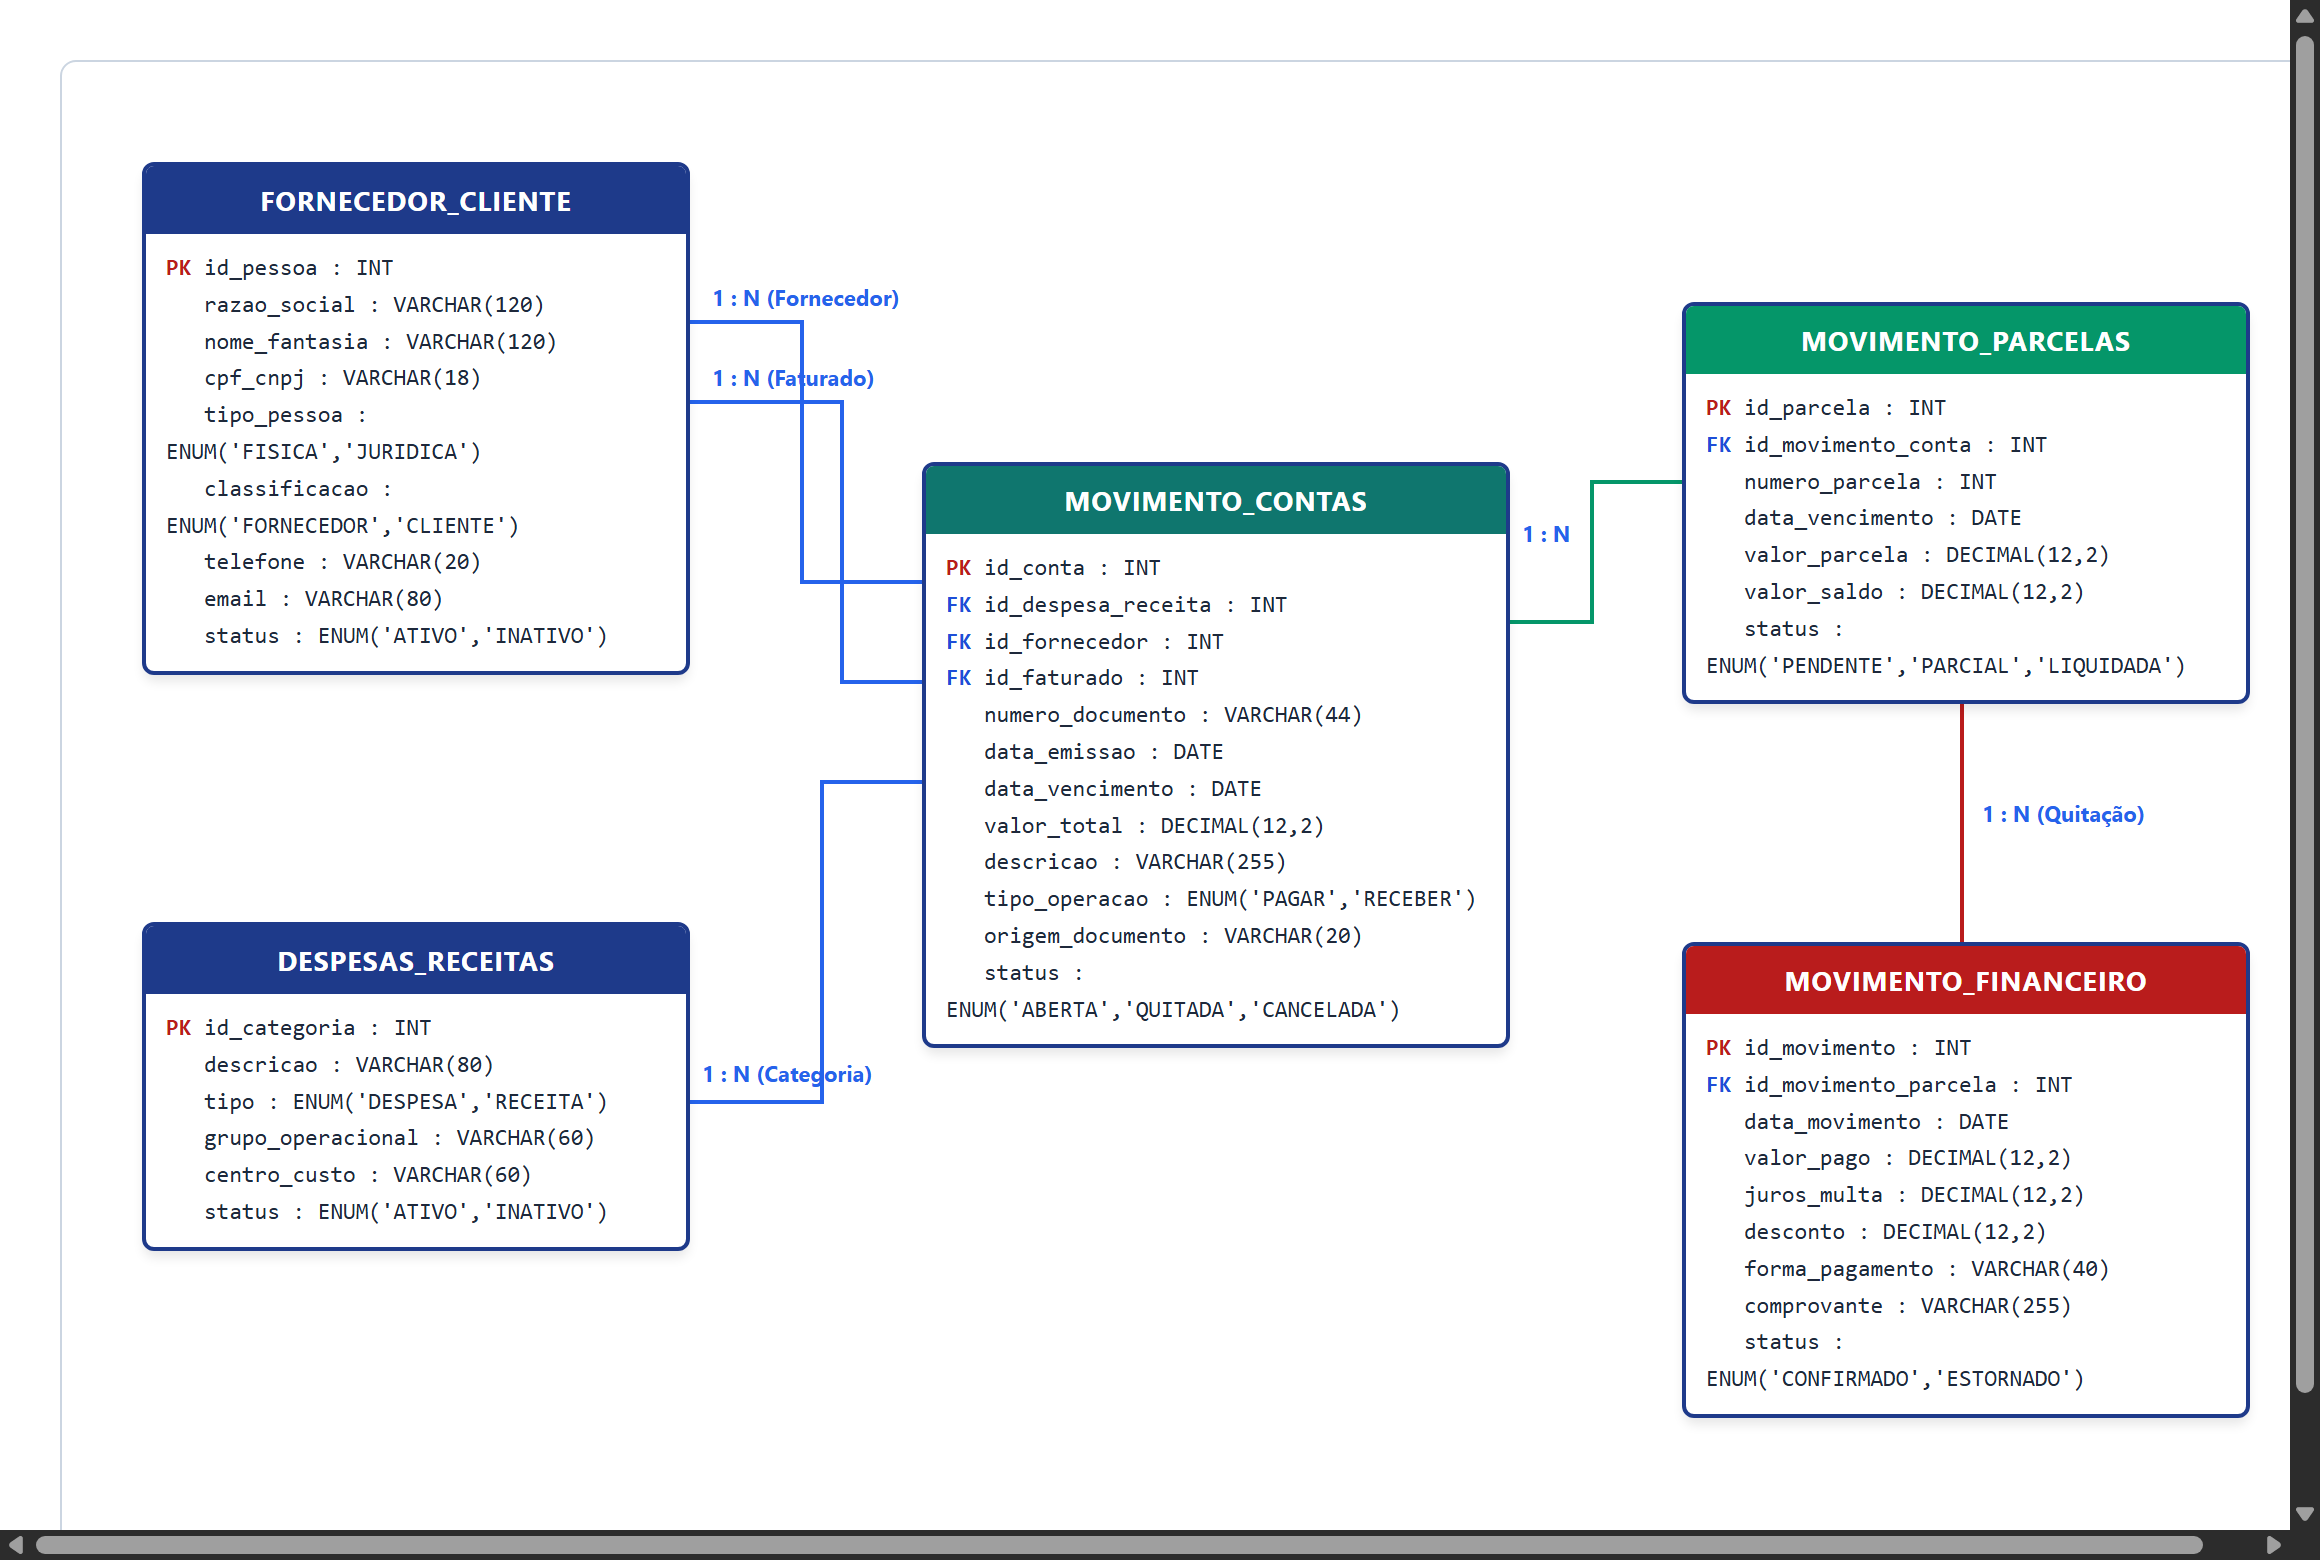
\includegraphics[width=0.96\textwidth]{assets/der.png}
	\caption{Diagrama Entidade-Relacionamento Oficial (5 Entidades e Chaves Estrangeiras)}
	\label{fig:der}
\end{figure}

\section{Diagramas de Sequência}

Os diagramas de sequência abaixo detalham a troca de mensagens orientada a objetos entre as camadas do sistema, com a mensagem final de confirmação retornando ao ator.

\subsection{Sequência 1: Movimentação Financeira e Quitação de Parcela}

A Figura \ref{fig:seq_quitacao} demonstra o fluxo de baixa financeira de parcela.

\begin{figure}[H]
	\centering
	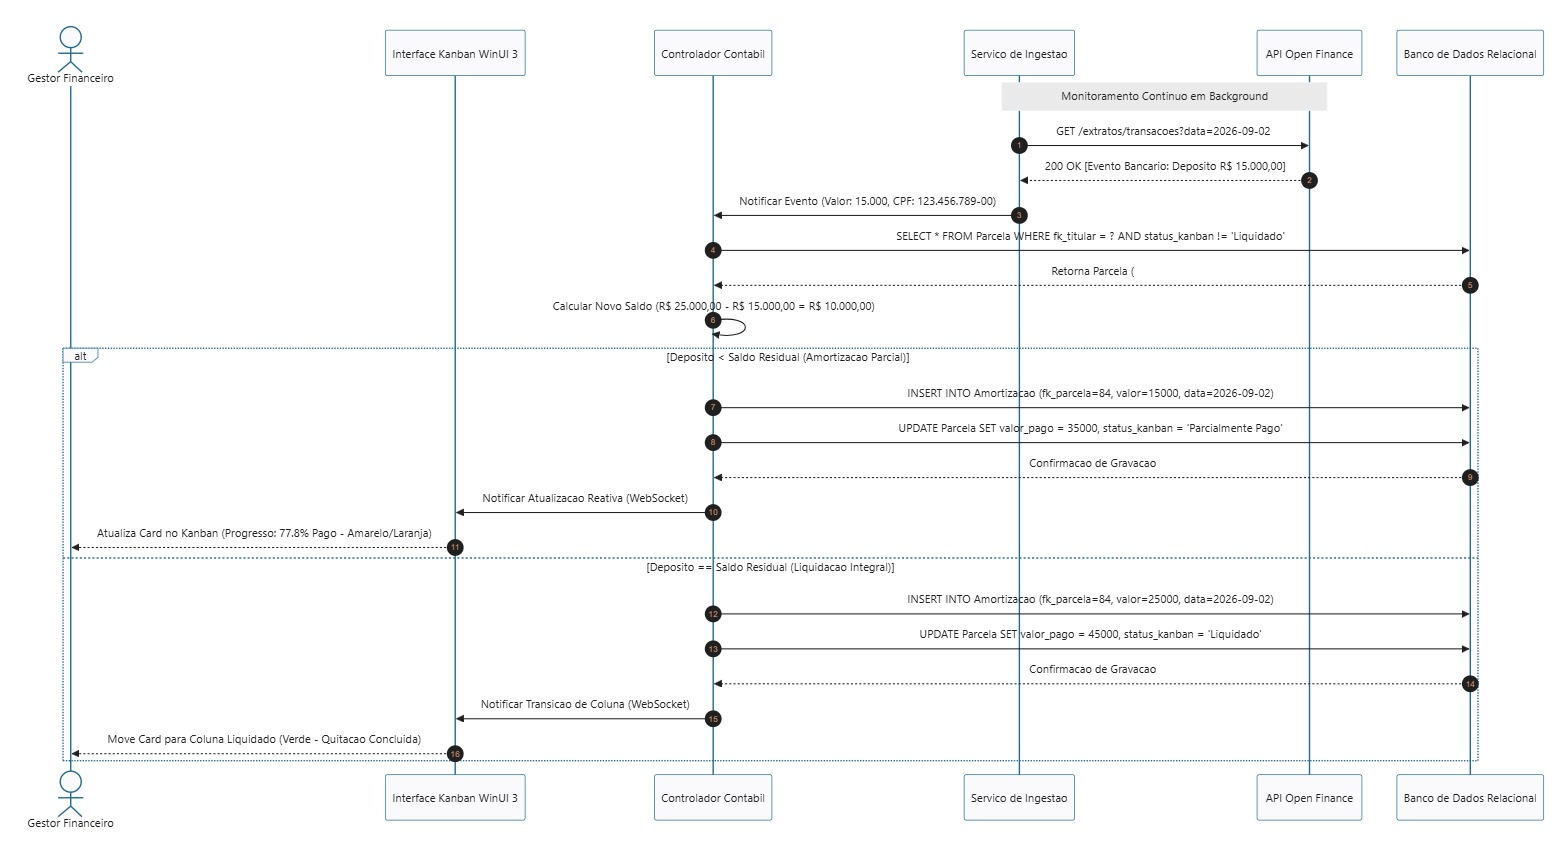
\includegraphics[width=0.92\textwidth]{assets/seq_quitacao.png}
	\caption{Diagrama de Sequência — Movimentação Financeira e Baixa de Parcela}
	\label{fig:seq_quitacao}
\end{figure}

\subsection{Sequência 2: Ingestão de Documento e Extração de Dados}

A Figura \ref{fig:seq_extracao} apresenta o fluxo orientado a objetos para upload do documento PDF e retorno dos dados extraídos para o usuário.

\begin{figure}[H]
	\centering
	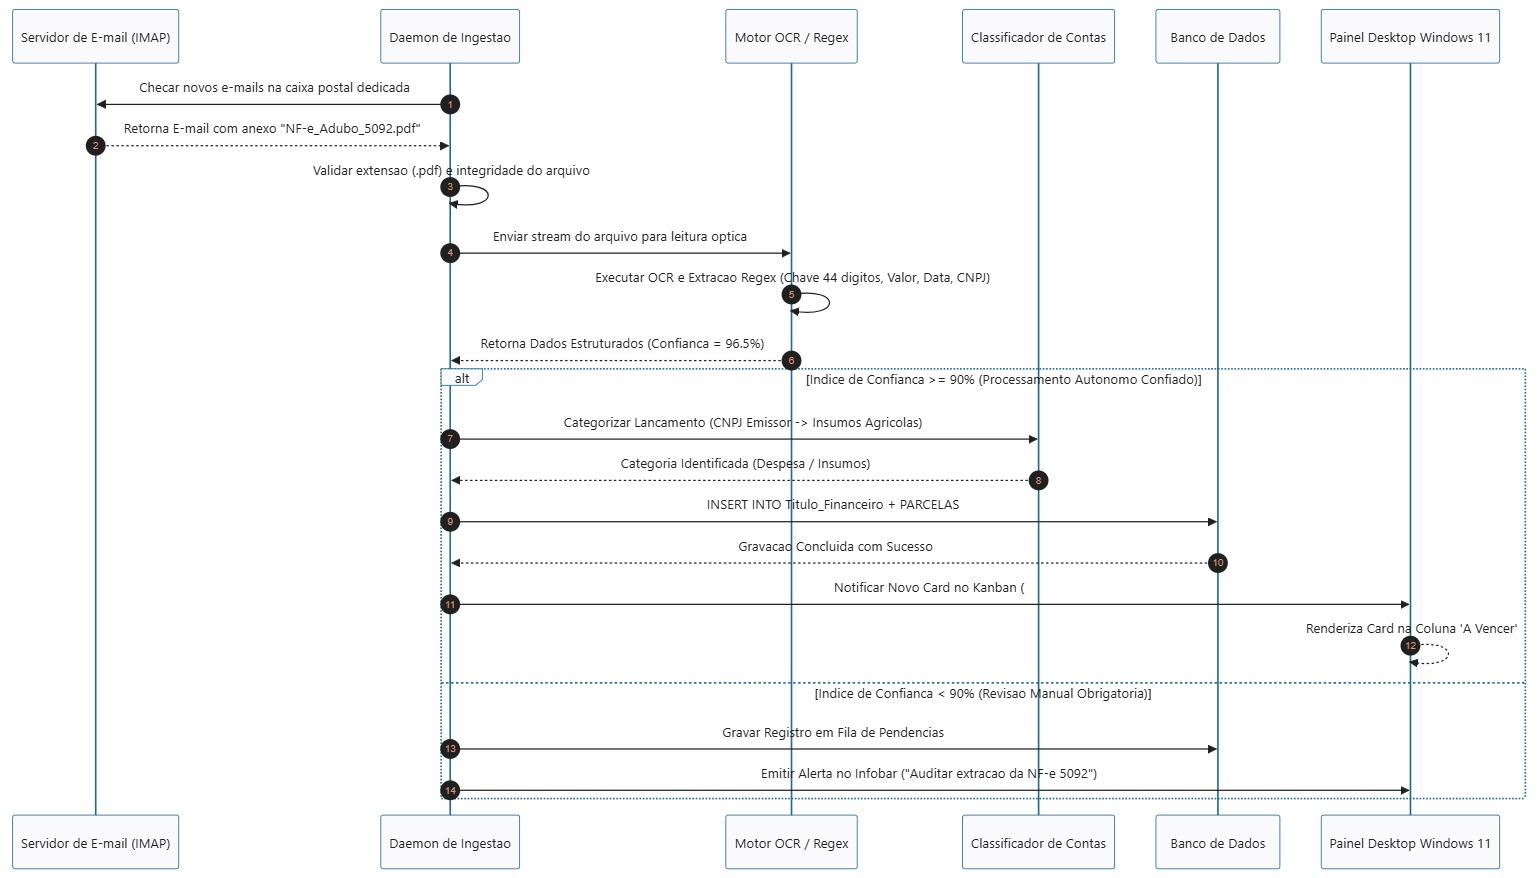
\includegraphics[width=0.92\textwidth]{assets/seq_extracao.png}
	\caption{Diagrama de Sequência — Upload e Extração de Dados do Documento}
	\label{fig:seq_extracao}
\end{figure}

% ==========================================================
% ANEXO 1: GANTTPROJECT
% ==========================================================
\chapter*{ANEXO 1: CRONOGRAMA GANTTPROJECT}
\addcontentsline{toc}{chapter}{ANEXO 1: CRONOGRAMA GANTTPROJECT}

O cronograma de execução do projeto foi estruturado com base nas 7 funções essenciais utilizando a ferramenta \textbf{GanttProject}. A Tabela \ref{tab:gantt} detalha as etapas, durações e predecessoras, enquanto a Figura \ref{fig:gantt} ilustra a visualização gráfica gerada.

\begin{table}[H]
	\centering
	\small
	\caption{Estrutura de Atividades do Projeto (GanttProject)}
	\label{tab:gantt}
	\begin{tabularx}{\textwidth}{c p{6cm} c c p{2.5cm}}
		\toprule
		\textbf{ID} & \textbf{Nome da Tarefa} & \textbf{Duração} & \textbf{Início} & \textbf{Predecessoras} \\
		\midrule
		1 & Elicitação de Requisitos e Modelagem DER & 5 dias & 01/09/2026 & - \\
		2 & RF01: Manter Fornecedor / Cliente & 7 dias & 08/09/2026 & 1 \\
		3 & RF02: Manter Despesas / Receitas & 6 dias & 16/09/2026 & 1 \\
		4 & RF06: Fazer Upload do Documento & 4 dias & 23/09/2026 & 1 \\
		5 & RF07: Extrair Dados do Documento & 8 dias & 28/09/2026 & 4 \\
		6 & RF03: Manter MovimentoContas & 8 dias & 07/10/2026 & 2, 3 \\
		7 & RF04: Manter MovimentoParcelas & 7 dias & 16/10/2026 & 6 \\
		8 & RF05: Manter MovimentoFinanceiro (Quitação) & 8 dias & 24/10/2026 & 7 \\
		9 & Homologação e Testes de Integração & 6 dias & 03/11/2026 & 5, 8 \\
		10 & Marco: Entrega Oficial do Sistema & 0 dias & 10/11/2026 & 9 \\
		\bottomrule
	\end{tabularx}
\end{table}

\begin{figure}[H]
	\centering
	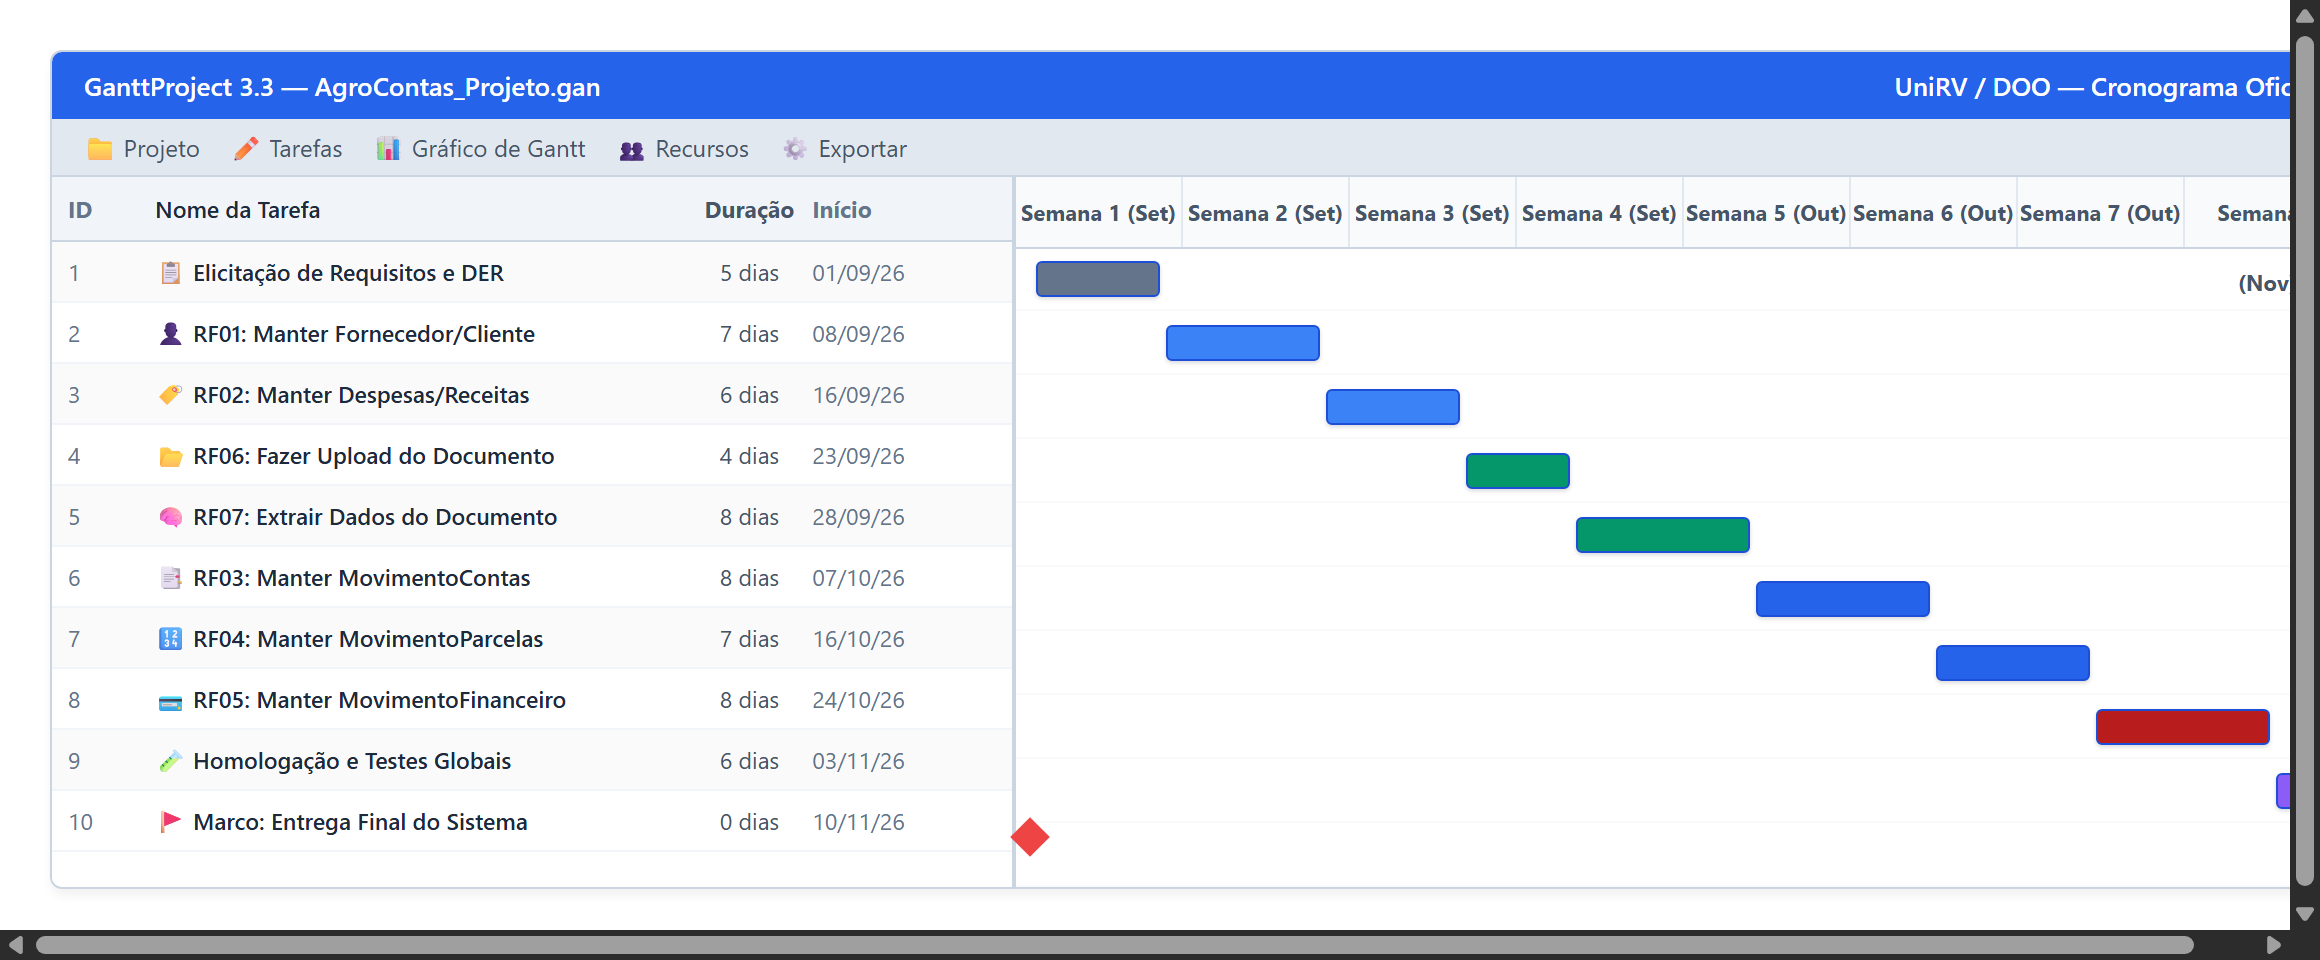
\includegraphics[width=0.96\textwidth]{assets/gantt.png}
	\caption{Cronograma de Execução Física — Exportação GanttProject}
	\label{fig:gantt}
\end{figure}

% ==========================================================
% ANEXO 2: ESPECIFICAÇÃO DOS REQUISITOS FUNCIONAIS
% ==========================================================
\chapter*{ANEXO 2: ESPECIFICAÇÃO DOS REQUISITOS FUNCIONAIS}
\addcontentsline{toc}{chapter}{ANEXO 2: ESPECIFICAÇÃO DOS REQUISITOS FUNCIONAIS}

Em atendimento rigoroso à avaliação do professor, este anexo apresenta a \textbf{especificação formal de cada um dos 7 requisitos funcionais (RF01 a RF07)}, acompanhada de seu respectivo protótipo de tela. 

Para todas as funcionalidades de manutenção (\textbf{MANTER}), a especificação adota como padrão mandatário a \textbf{tela de listagem/consulta como a primeira tela apresentada ao usuário}, dispondo de filtros de busca e botões de ação (\textit{Consultar}, \textit{Incluir}, \textit{Alterar}, \textit{Desativar}).

% ----------------------------------------------------------
% RF01
% ----------------------------------------------------------
\section*{RF01 — Manter Fornecedor / Cliente}

\subsection*{1. Breve Descrição}
Permite consultar, incluir, alterar e desativar os cadastros de fornecedores e clientes/titulares do agronegócio.

\subsection*{2. Atores}
Gestor Financeiro Rural (Usuário do Sistema).

\subsection*{3. Fluxo de Eventos}
\subsubsection*{3.1. Fluxo Básico (Listagem / Consulta — Primeira Tela)}
\begin{enumerate}[leftmargin=0.8cm]
	\item O ator acessa o menu \textbf{"Cadastros $\rightarrow$ Fornecedores e Clientes"};
	\item O sistema exibe a \textbf{tela de listagem inicial} contendo os seguintes campos de filtro:
	\begin{itemize}
		\item \textit{Razão Social / Nome Fantasia}: Texto, opcional, padrão em branco;
		\item \textit{CPF / CNPJ}: Texto com máscara, opcional;
		\item \textit{Classificação}: Caixa de seleção (\textit{Todos}, \textit{Fornecedor}, \textit{Cliente/Titular});
		\item \textit{Somente Ativos}: Caixa de checagem, padrão marcado (\textit{Sim});
	\end{itemize}
	\item O ator aciona a opção \textbf{"Consultar"};
	\item O sistema recupera os registros e exibe a tabela em DataGrid contendo as colunas: \textit{Sel, Cód, Razão Social / Nome, Nome Fantasia, CPF/CNPJ, Tipo, Telefone, Status};
	\item O sistema disponibiliza os botões de ação: \textbf{Consultar}, \textbf{Incluir Novo}, \textbf{Alterar Selecionado} e \textbf{Desativar};
	\item O caso de uso encerra a consulta aguardando seleção do operador.
\end{enumerate}

\subsubsection*{3.2. Fluxo Alternativo A1: Inclusão}
\begin{enumerate}[leftmargin=0.8cm]
	\item No passo 5 do fluxo básico, o ator clica em \textbf{"Incluir Novo"};
	\item O sistema exibe o formulário de cadastro com os campos: Razão Social (*), Nome Fantasia, CPF/CNPJ (*), Tipo de Pessoa (*), Classificação (*), Telefone e E-mail;
	\item O ator preenche os dados e aciona \textbf{"Salvar"};
	\item O sistema valida a unicidade do CPF/CNPJ, persiste o registro como \textbf{ATIVO} e retorna à tela de listagem atualizada.
\end{enumerate}

\subsection*{4. Protótipo de Tela do RF01}
A Figura \ref{fig:proto_rf01} ilustra a tela de listagem inicial do gerenciamento de fornecedores e clientes.

\begin{figure}[H]
	\centering
	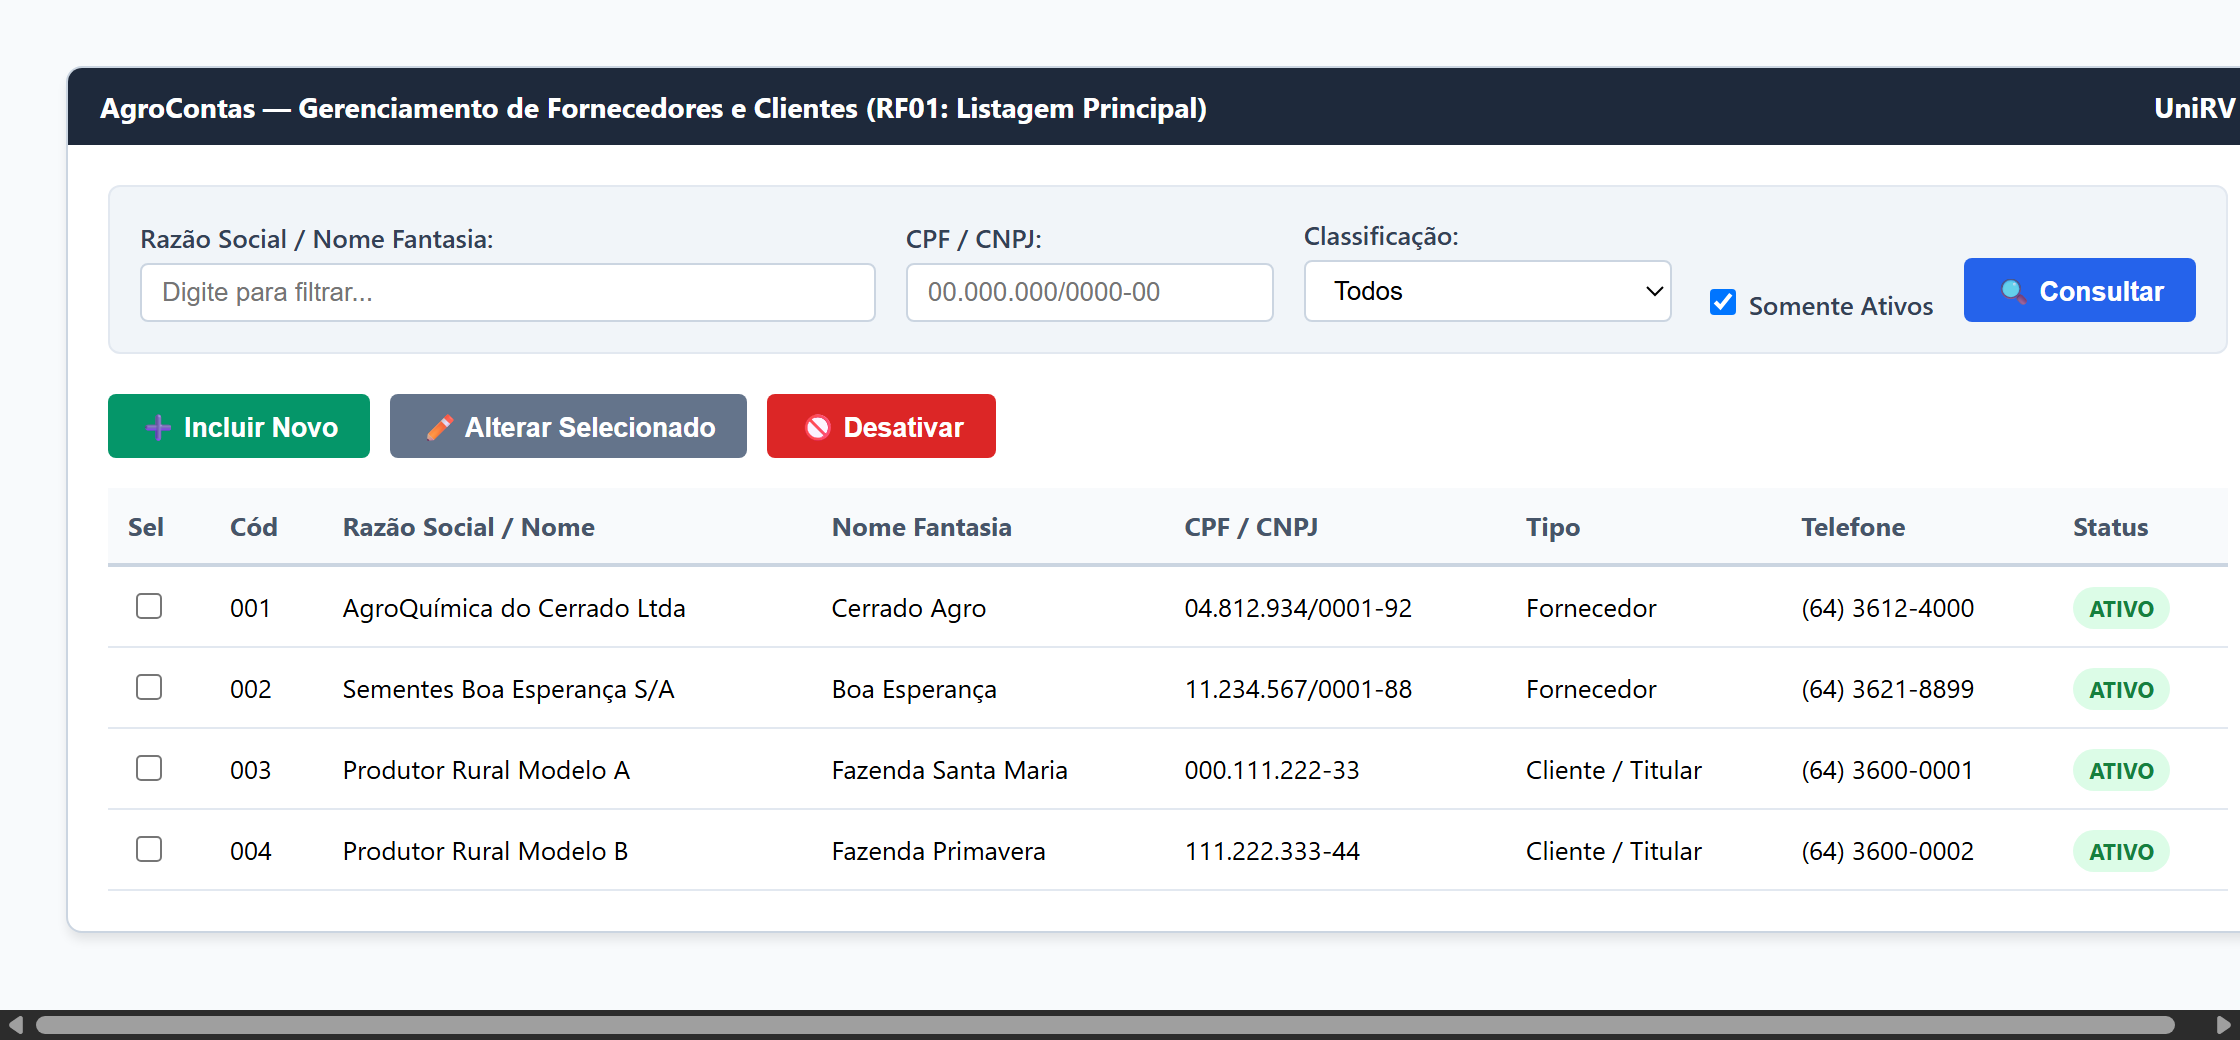
\includegraphics[width=0.94\textwidth]{assets/proto_rf01_fornecedor.png}
	\caption{Protótipo de Tela RF01 — Listagem Principal de Fornecedores e Clientes}
	\label{fig:proto_rf01}
\end{figure}

% ----------------------------------------------------------
% RF02
% ----------------------------------------------------------
\clearpage
\section*{RF02 — Manter Despesas / Receitas}

\subsection*{1. Breve Descrição}
Gerencia as categorias contábeis e centros de custo do plano de contas rural.

\subsection*{2. Atores}
Gestor Financeiro Rural.

\subsection*{3. Fluxo de Eventos}
\subsubsection*{3.1. Fluxo Básico (Listagem / Consulta — Primeira Tela)}
\begin{enumerate}[leftmargin=0.8cm]
	\item O ator acessa o menu \textbf{"Cadastros $\rightarrow$ Plano de Contas (Despesas/Receitas)"};
	\item O sistema exibe a \textbf{tela de listagem inicial} com filtros por \textit{Descrição da Categoria}, \textit{Tipo} (Despesa ou Receita) e \textit{Centro de Custo};
	\item O ator aciona \textbf{"Consultar"};
	\item O sistema apresenta o DataGrid contendo: \textit{Cód, Descrição da Categoria, Tipo, Grupo Operacional, Centro de Custo e Status};
	\item O sistema disponibiliza os botões: \textbf{Consultar}, \textbf{Nova Despesa/Receita} e \textbf{Alterar Categoria}.
\end{enumerate}

\subsection*{4. Protótipo de Tela do RF02}
A Figura \ref{fig:proto_rf02} apresenta a tela de listagem inicial para o plano de contas.

\begin{figure}[H]
	\centering
	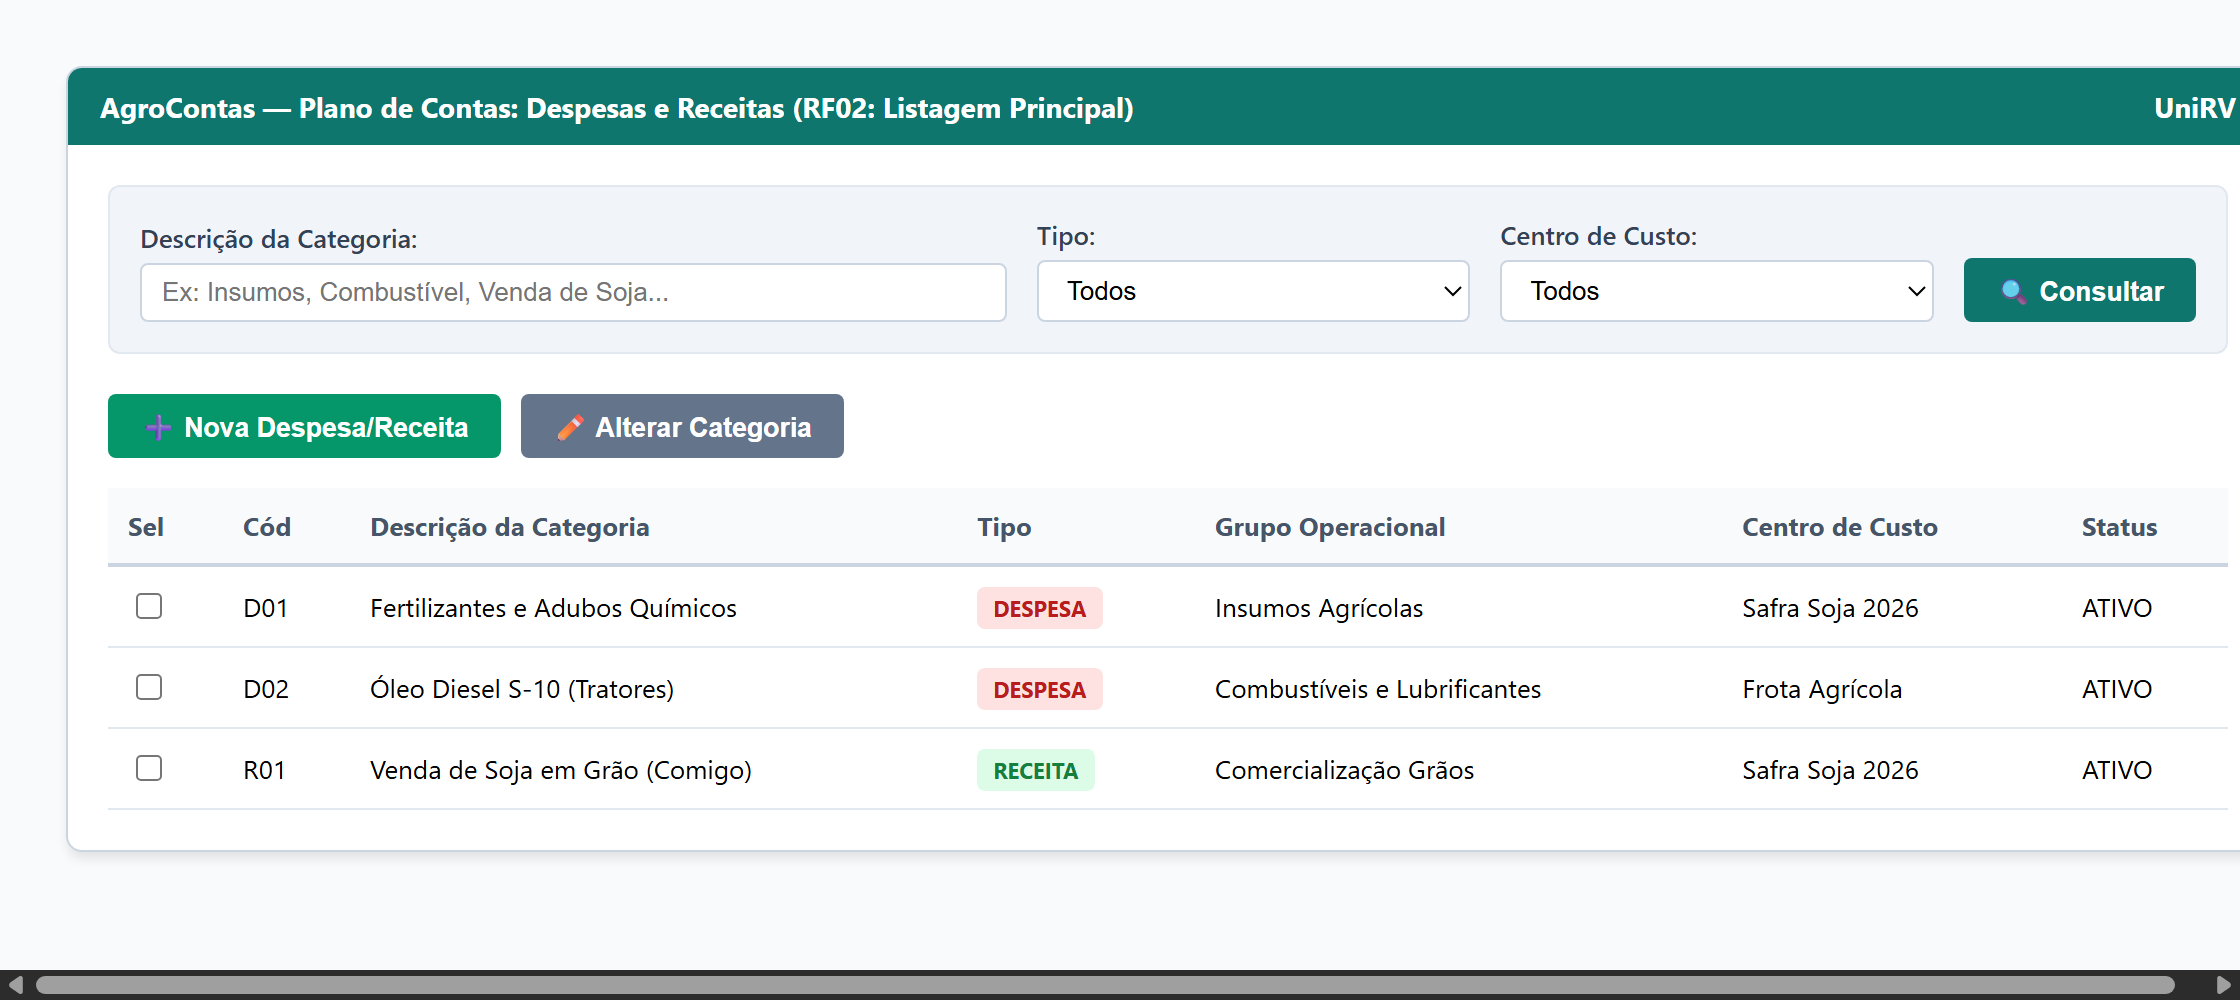
\includegraphics[width=0.94\textwidth]{assets/proto_rf02_despesas.png}
	\caption{Protótipo de Tela RF02 — Listagem Principal de Despesas e Receitas}
	\label{fig:proto_rf02}
\end{figure}

% ----------------------------------------------------------
% RF03
% ----------------------------------------------------------
\clearpage
\section*{RF03 — Manter MovimentoContas}

\subsection*{1. Breve Descrição}
Controla os títulos de Contas a Pagar e Contas a Receber, associando o documento fiscal às partes envolvidas (Fornecedor e Faturado) e à respectiva categoria de despesa.

\subsection*{2. Atores}
Gestor Financeiro Rural.

\subsection*{3. Fluxo de Eventos}
\subsubsection*{3.1. Fluxo Básico (Listagem / Consulta — Primeira Tela)}
\begin{enumerate}[leftmargin=0.8cm]
	\item O ator seleciona o menu \textbf{"Financeiro $\rightarrow$ Movimento de Contas"};
	\item O sistema abre a \textbf{tela de listagem principal} contendo os filtros: \textit{Nº Documento/NF-e}, \textit{Fornecedor}, \textit{Faturado/Titular} e \textit{Tipo de Operação} (Pagar ou Receber);
	\item O ator clica em \textbf{"Consultar"};
	\item O sistema lista as contas no DataGrid com as colunas: \textit{Sel, Cód, Nº Documento, Fornecedor (FK), Faturado (FK), Despesa (FK), Emissão, Vencimento, Valor Total e Status};
	\item Estão disponíveis os botões: \textbf{Consultar}, \textbf{Lançar Nova Conta}, \textbf{Ver Parcelas da Conta} e \textbf{Editar Título}.
\end{enumerate}

\subsection*{4. Protótipo de Tela do RF03}
A Figura \ref{fig:proto_rf03} apresenta a tela de listagem principal de contas a pagar e receber.

\begin{figure}[H]
	\centering
	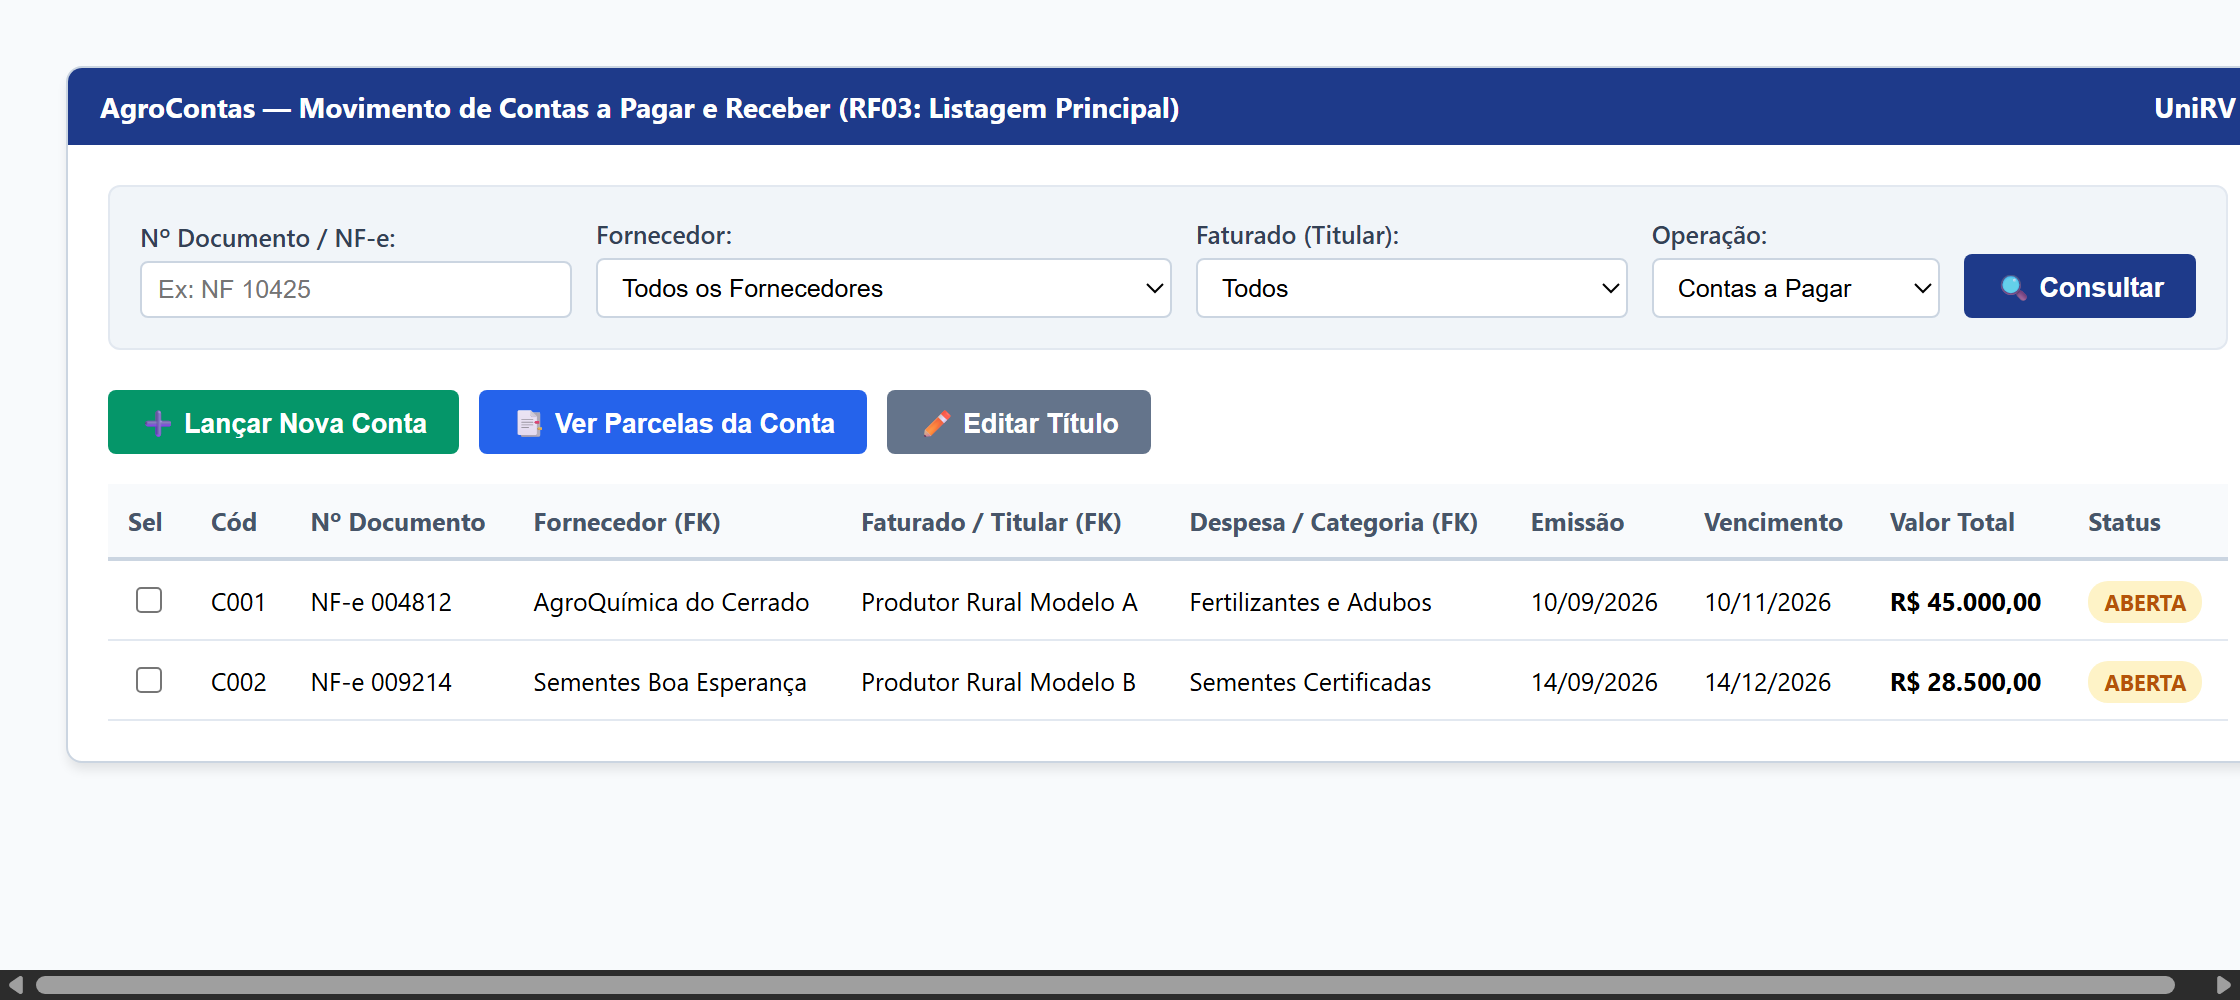
\includegraphics[width=0.94\textwidth]{assets/proto_rf03_contas.png}
	\caption{Protótipo de Tela RF03 — Listagem Principal de Movimento de Contas}
	\label{fig:proto_rf03}
\end{figure}

% ----------------------------------------------------------
% RF04
% ----------------------------------------------------------
\clearpage
\section*{RF04 — Manter MovimentoParcelas}

\subsection*{1. Breve Descrição}
Gerencia as parcelas vinculadas a cada conta, controlando vencimentos parciais, amortizações sucessivas e liquidação de saldos.

\subsection*{2. Atores}
Gestor Financeiro Rural.

\subsection*{3. Fluxo de Eventos}
\subsubsection*{3.1. Fluxo Básico (Listagem / Consulta — Primeira Tela)}
\begin{enumerate}[leftmargin=0.8cm]
	\item O ator seleciona a opção \textbf{"Contas / Parcelamentos"} ou clica em \textbf{"Ver Parcelas"} a partir de uma conta selecionada;
	\item O sistema exibe o DataGrid com a relação de parcelas: \textit{Identificação da Parcela, Titular, Valor da Parcela, Vencimento e Status};
	\item O ator seleciona uma parcela e clica em \textbf{"Amortizar / Detalhar"};
	\item O sistema exibe o modal mestre-detalhe com o histórico de amortizações parciais efetuadas sobre a parcela.
\end{enumerate}

\subsection*{4. Protótipos de Tela do RF04}
As Figuras \ref{fig:proto_rf04_grid} e \ref{fig:proto_rf04_modal} exibem a tela de listagem de parcelas e o respectivo formulário mestre-detalhe de amortizações fracionadas.

\begin{figure}[H]
	\centering
	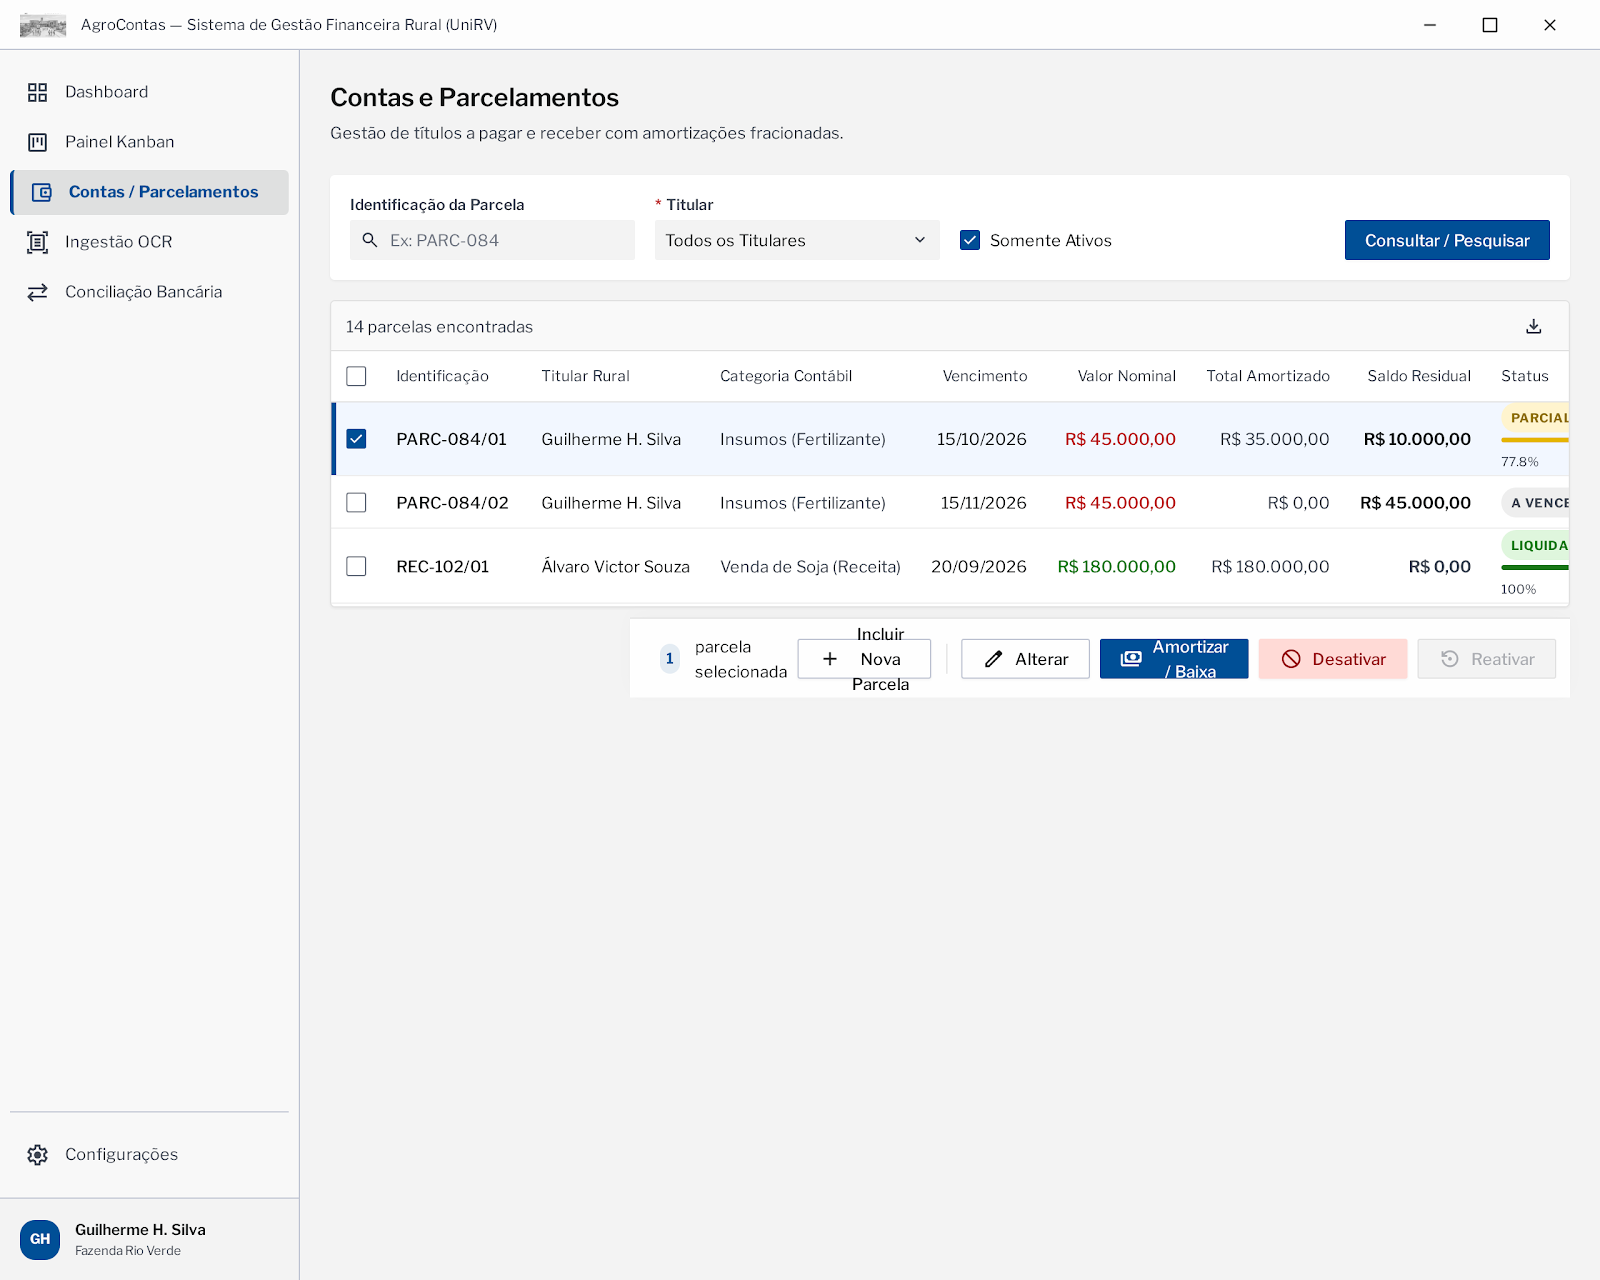
\includegraphics[width=0.92\textwidth]{assets/proto_rf04_listagem.png}
	\caption{Protótipo de Tela RF04 — Listagem Principal de Parcelas (DataGrid)}
	\label{fig:proto_rf04_grid}
\end{figure}

\begin{figure}[H]
	\centering
	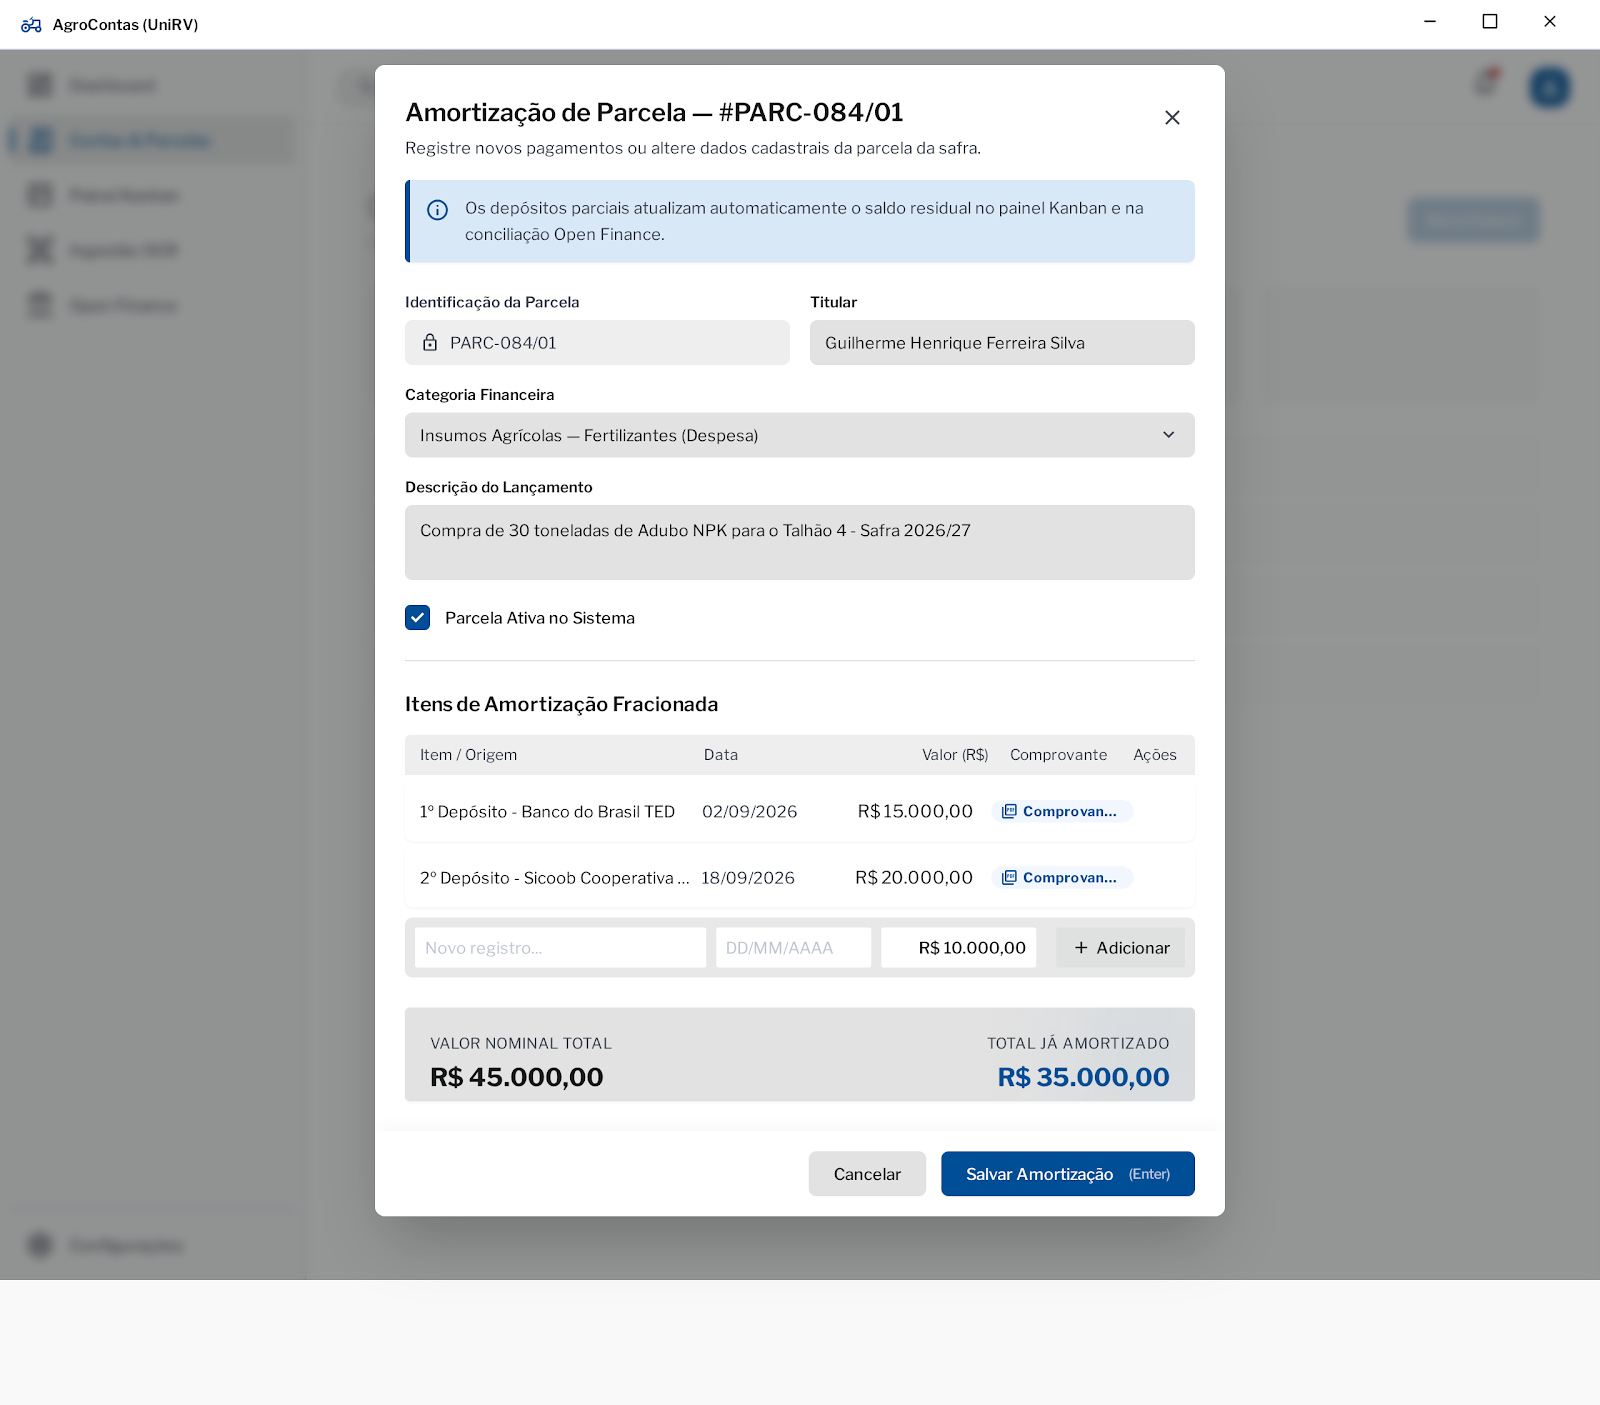
\includegraphics[width=0.92\textwidth]{assets/proto_rf04_detalhe.png}
	\caption{Protótipo de Tela RF04 — Modal Mestre-Detalhe de Amortização de Parcela}
	\label{fig:proto_rf04_modal}
\end{figure}

% ----------------------------------------------------------
% RF05
% ----------------------------------------------------------
\clearpage
\section*{RF05 — Manter MovimentoFinanceiro (Quitação)}

\subsection*{1. Breve Descrição}
Registra e audita as baixas e liquidações financeiras efetuadas sobre as parcelas em aberto, informando datas de pagamento, valores líquidos, juros/multas e meios de transação.

\subsection*{2. Atores}
Gestor Financeiro Rural.

\subsection*{3. Fluxo de Eventos}
\subsubsection*{3.1. Fluxo Básico (Listagem / Consulta — Primeira Tela)}
\begin{enumerate}[leftmargin=0.8cm]
	\item O ator navega até o menu \textbf{"Financeiro $\rightarrow$ Movimentações e Quitações"};
	\item O sistema apresenta a \textbf{tela de listagem inicial} com filtros de período (\textit{Data De} / \textit{Data Até}) e \textit{Forma de Pagamento} (PIX, Boleto, TED);
	\item O sistema exibe os pagamentos confirmados no DataGrid com as colunas: \textit{Cód Mov, Parcela Vinculada (FK), Data Pagamento, Valor Pago, Juros/Multa, Desconto, Forma de Pagamento e Status};
	\item O sistema disponibiliza os botões: \textbf{Realizar Nova Quitação / Baixa} e \textbf{Visualizar Comprovante}.
\end{enumerate}

\subsection*{4. Protótipo de Tela do RF05}
A Figura \ref{fig:proto_rf05} apresenta a tela de listagem principal de movimentações financeiras e baixas.

\begin{figure}[H]
	\centering
	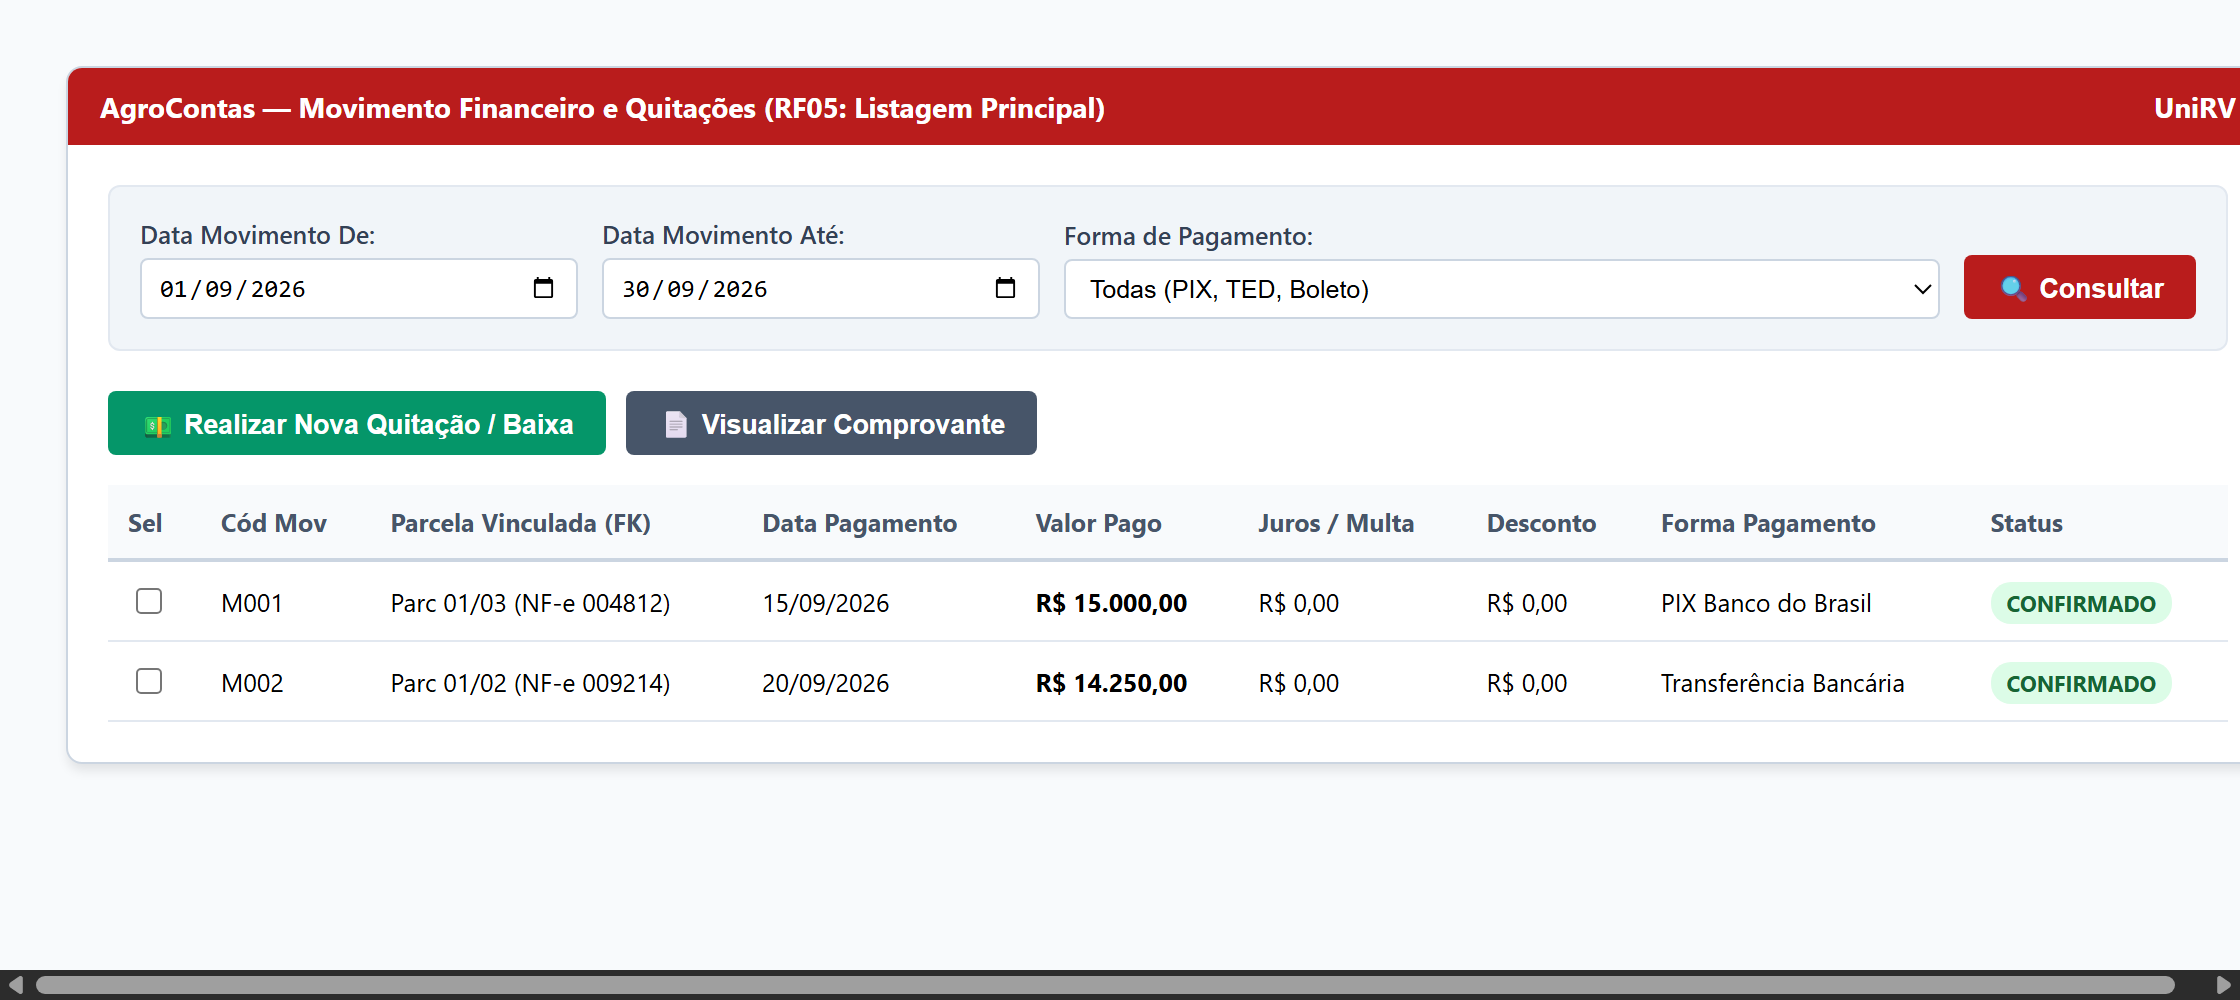
\includegraphics[width=0.94\textwidth]{assets/proto_rf05_quitacao.png}
	\caption{Protótipo de Tela RF05 — Listagem Principal de Quitações e Baixas Financeiras}
	\label{fig:proto_rf05}
\end{figure}

% ----------------------------------------------------------
% RF06
% ----------------------------------------------------------
\clearpage
\section*{RF06 — Fazer Upload do Documento}

\subsection*{1. Breve Descrição}
Disponibiliza mecanismo de upload de arquivos digitais em formato PDF (faturas, DANFE, notas fiscais de insumos ou prestação de serviços agrícolas).

\subsection*{2. Atores}
Gestor Financeiro Rural.

\subsection*{3. Fluxo de Eventos}
\subsubsection*{3.1. Fluxo Básico}
\begin{enumerate}[leftmargin=0.8cm]
	\item O ator acessa o menu \textbf{"Documentos $\rightarrow$ Upload de Notas Fiscais"};
	\item O sistema exibe a tela de carregamento contendo uma área de arrastar-e-soltar (\textit{Drag \& Drop}) e botão de seleção de arquivo local;
	\item O ator arrasta ou seleciona um arquivo em formato PDF com tamanho de até 10MB;
	\item O sistema valida a extensão e integridade do arquivo e exibe a pré-visualização;
	\item O ator clica em \textbf{"Processar e Extrair Dados"};
	\item O sistema envia o arquivo para a esteira de análise automática (disparando o RF07).
\end{enumerate}

\subsection*{4. Protótipo de Tela do RF06}
A Figura \ref{fig:proto_rf06} apresenta a tela de upload e seleção de documentos fiscais em PDF.

\begin{figure}[H]
	\centering
	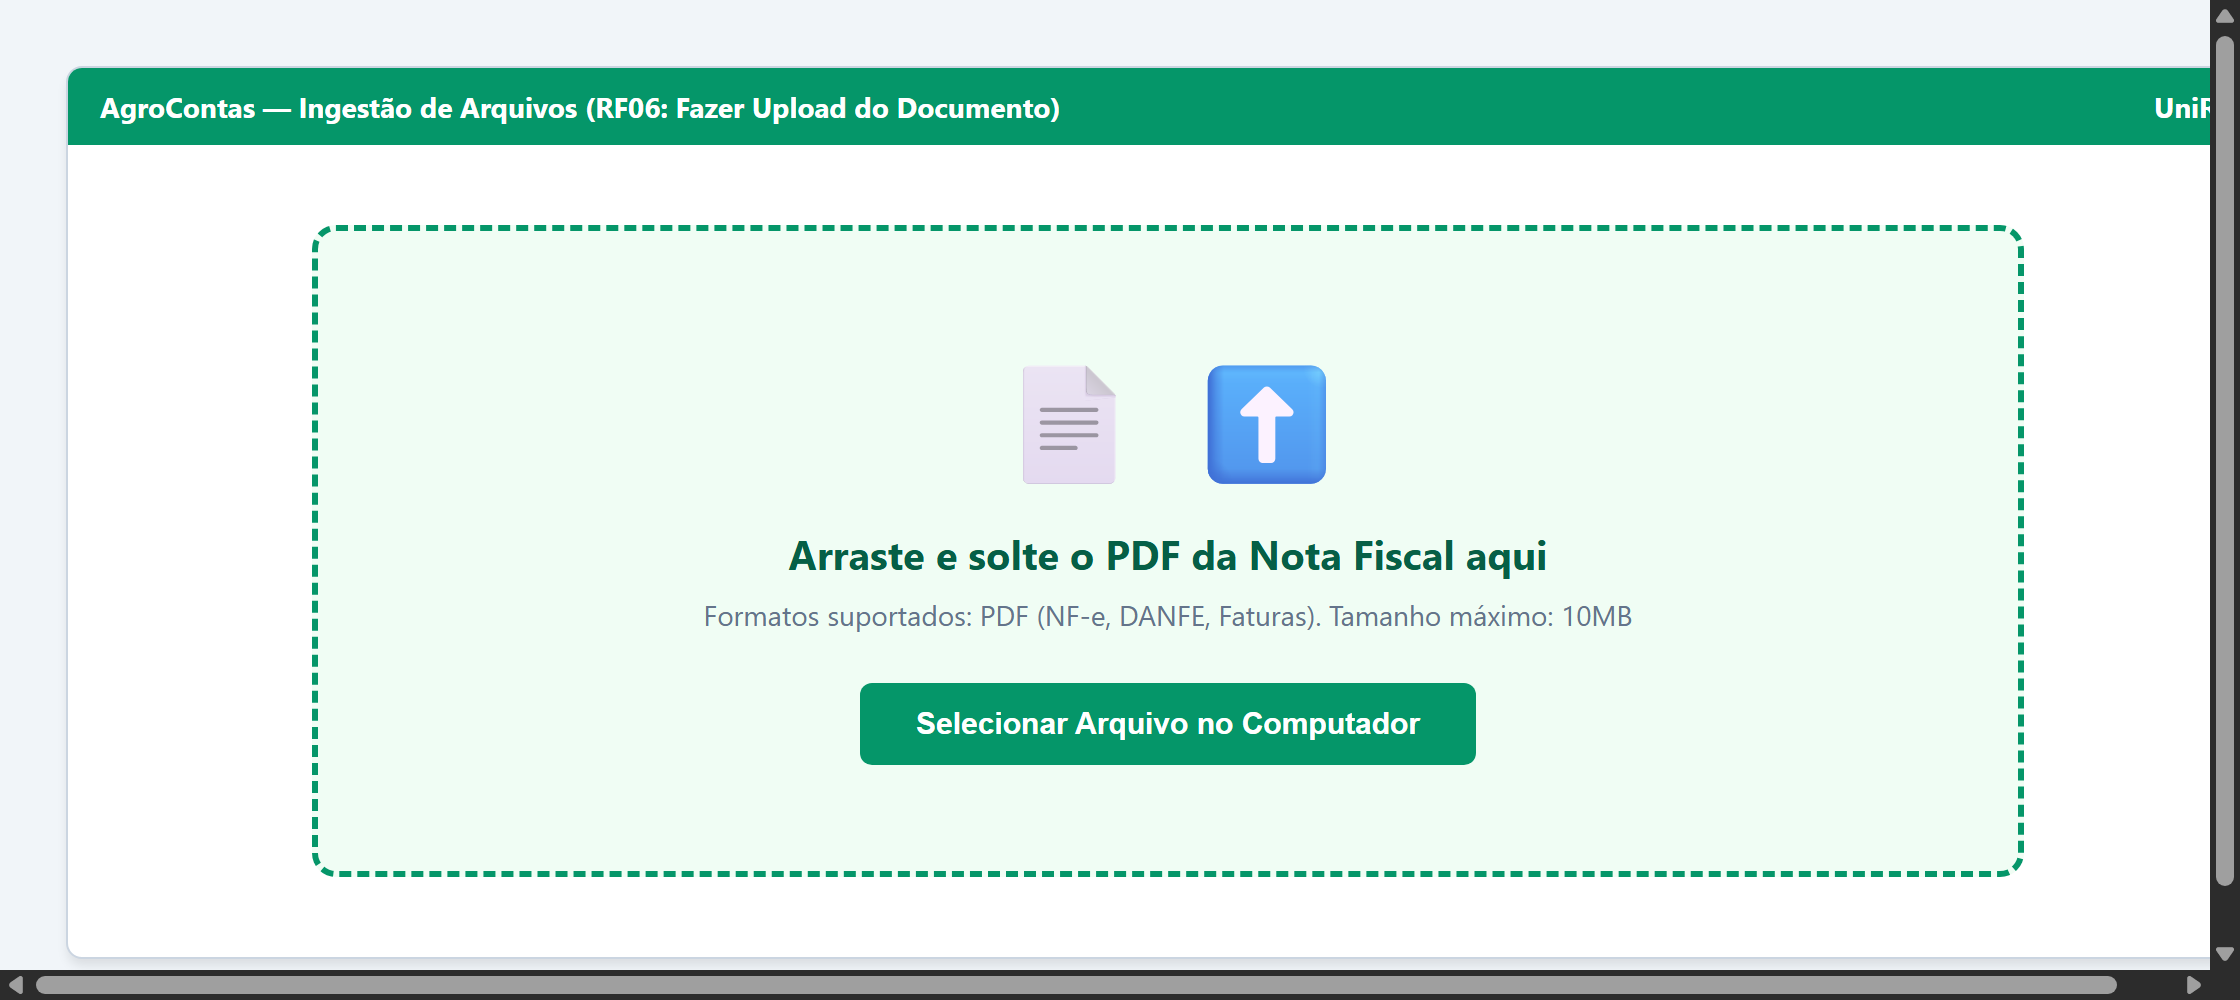
\includegraphics[width=0.94\textwidth]{assets/proto_rf06_upload.png}
	\caption{Protótipo de Tela RF06 — Interface de Upload de Documento PDF}
	\label{fig:proto_rf06}
\end{figure}

% ----------------------------------------------------------
% RF07
% ----------------------------------------------------------
\clearpage
\section*{RF07 — Extrair Dados do Documento}

\subsection*{1. Breve Descrição}
Executa a interpretação semântica do documento fiscal em PDF, extraindo dados do emitente/fornecedor, destinatário/faturado, número da nota, itens, valores totais e datas das parcelas para revisão do gestor.

\subsection*{2. Atores}
Serviço de IA / OCR (Ator Secundário) e Gestor Financeiro Rural.

\subsection*{3. Fluxo de Eventos}
\subsubsection*{3.1. Fluxo Básico}
\begin{enumerate}[leftmargin=0.8cm]
	\item O sistema recebe o documento submetido no RF06;
	\item O motor de inteligência/extração processa o texto e estrutura as entidades de negócio;
	\item O sistema apresenta ao usuário a tela em formato \textbf{Split-View}: documento PDF original na lateral esquerda e os campos extraídos preenchidos na lateral direita;
	\item O gestor valida ou ajusta os dados conferidos;
	\item O gestor clica em \textbf{"Confirmar e Gerar Conta"};
	\item O sistema grava os registros nas tabelas correspondentes (\textit{MovimentoContas} e \textit{MovimentoParcelas}).
\end{enumerate}

\subsection*{4. Protótipo de Tela do RF07}
A Figura \ref{fig:proto_rf07} apresenta a interface de conferência e auditoria de dados extraídos em tela dividida.

\begin{figure}[H]
	\centering
	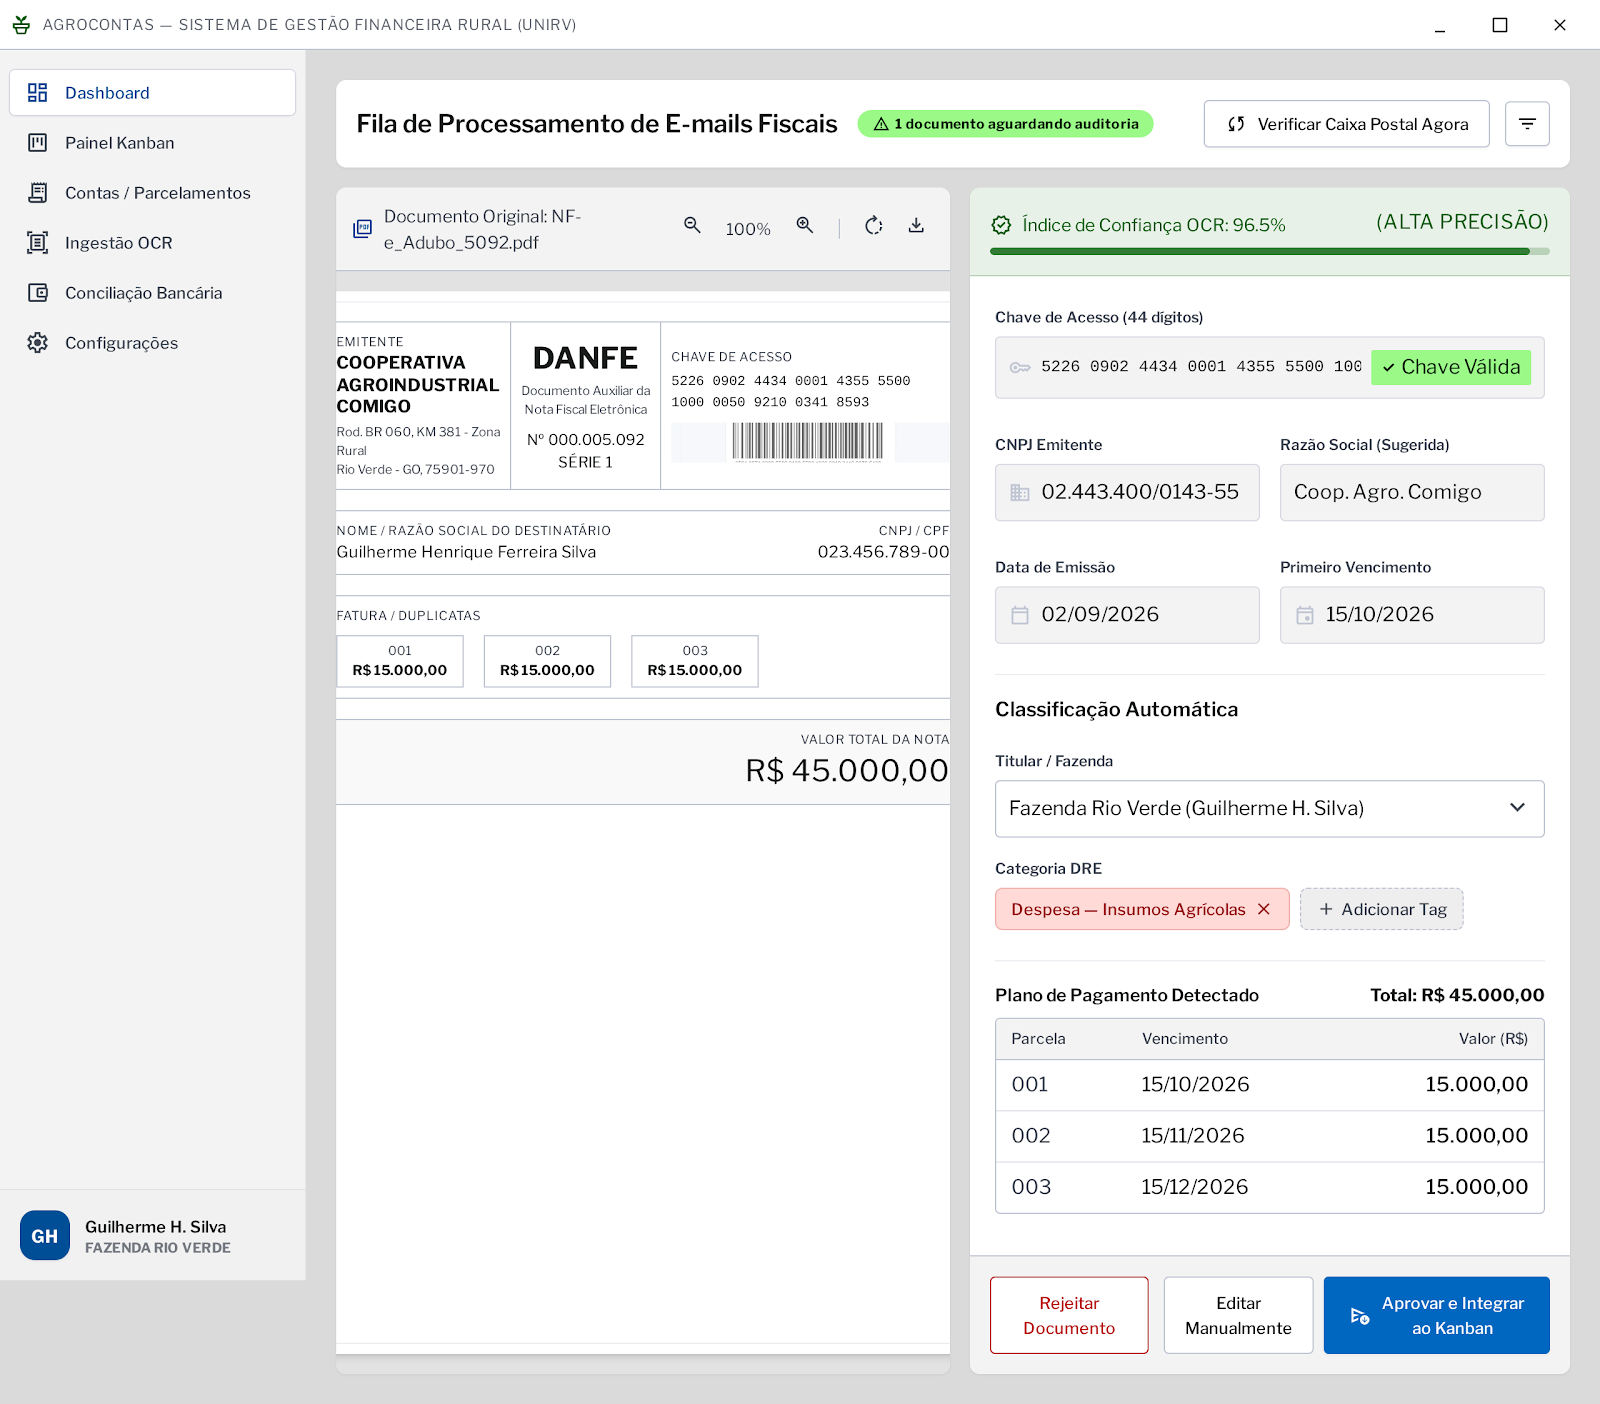
\includegraphics[width=0.94\textwidth]{assets/proto_rf07_extracao.png}
	\caption{Protótipo de Tela RF07 — Interface Split-View de Extração e Auditoria}
	\label{fig:proto_rf07}
\end{figure}

% ==========================================================
% REFERÊNCIAS
% ==========================================================
\clearpage
\begin{thebibliography}{99}
	\bibitem{abnt14724} ASSOCIAÇÃO BRASILEIRA DE NORMAS TÉCNICAS. \textbf{NBR 14724}: Informação e documentação — Trabalhos acadêmicos — Apresentação. Rio de Janeiro: ABNT, 2011.
	\bibitem{ieee830} IEEE COMPUTER SOCIETY. \textbf{IEEE Std 830-1998}: IEEE Recommended Practice for Software Requirements Specifications. Piscataway, NJ: IEEE, 1998.
	\bibitem{iso29148} INTERNATIONAL ORGANIZATION FOR STANDARDIZATION. \textbf{ISO/IEC/IEEE 29148:2018}: Systems and software engineering — Life cycle processes — Requirements engineering. Geneva: ISO/IEC, 2018.
	\bibitem{pressman} PRESSMAN, Roger S.; MAXIM, Bruce R. \textbf{Engenharia de Software: Uma Abordagem Profissional}. 9. ed. Porto Alegre: AMGH, 2021.
	\bibitem{sommerville} SOMMERVILLE, Ian. \textbf{Engenharia de Software}. 10. ed. São Paulo: Pearson, 2019.
\end{thebibliography}

\end{document}
